% =====================================================================
% Morphological Efficiency in Multilingual Language Models
% Submission to Natural Language Processing (Cambridge University Press)
%
% TEMPLATE NOTE
% =============
% This file compiles standalone with `article`. Before submission, replace
% the document-class line below with the Cambridge NLP class (cambridge7A
% or equivalent, distributed via the journal's Overleaf template or via
% the "NLP LaTeX Files" download from the journal's Instructions for
% Contributors). The section structure, bibliography style, and figure
% references are written to be portable; only the preamble should need
% adjustment when swapping templates.
% =====================================================================

\documentclass[11pt, a4paper]{article}

% -- Packages -----------------------------------------------------------
\usepackage[utf8]{inputenc}
\usepackage[T1]{fontenc}
\usepackage{lmodern}
\usepackage[margin=2.5cm]{geometry}
\usepackage{amsmath, amssymb}
\usepackage{graphicx}
\usepackage{booktabs}
\usepackage{placeins}        % \FloatBarrier to pin floats inside subsections
\usepackage{natbib}          % author-date citations; Cambridge compatible
\usepackage{xcolor}
\usepackage{hyperref}
\hypersetup{colorlinks=true, citecolor=blue!60!black, linkcolor=blue!60!black, urlcolor=blue!60!black}
\usepackage{enumitem}
\usepackage{setspace}
\usepackage{csquotes}
% Arabic script support for the case-study section.
% When compiled under the Cambridge template, verify the correct package
% name and font configuration for polyglossia or arabtex.
\usepackage{fontspec}        % requires XeLaTeX or LuaLaTeX
\newfontfamily\arabicfont[Script=Arabic]{Amiri}   % fallback if Amiri unavailable
% -----------------------------------------------------------------------

\setlength{\parskip}{4pt}
\setlength{\parindent}{0pt}
\singlespacing

% Figure path
\graphicspath{{../figures/}}

% Title and authors
\title{%
Morphology-Aware Tokenization as a Capacity Lever: \\
Rethinking Scaling Laws for Morphologically Rich Languages
}

\author{%
Sameh AbuRadi\thanks{Corresponding author. ORCID: \href{https://orcid.org/0009-0008-0716-7598}{0009-0008-0716-7598}. Email: \href{mailto:Sameh.AbuRadi@CODE.Berlin}{Sameh.AbuRadi@CODE.Berlin}.} \\
\textit{CODE University of Applied Sciences, Berlin} \\
\textit{Supervised by Fabian Geier}
}

\date{Draft of \today}

\begin{document}
\maketitle

% -- Abstract -----------------------------------------------------------
\begin{abstract}
Transformer scaling laws (\emph{the empirical curves that predict how a language model's performance grows with its parameter count and the amount of text it is trained on}) are seemingly fitted on analytic-leaning languages such as English and Mandarin, whose words carry little grammatical marking on their written surface. This could genuinely be due to the fact that the AI market is dominated by China and Anglophone regions of the world at the time of writing. This paper asks whether languages at the opposite end of the typological spectrum, whose words inflect richly and write that inflection out in full, can turn their grammatical structure into a measurable computational efficiency factor.

The mechanism we study is \emph{grammar-aware tokenisation}. Instead of chopping text into frequent character fragments by statistics alone (\emph{byte-pair encoding, or BPE for short, which never consults grammar}), we hand the model a grammatical analysis of each word: its part of speech and the bundle of inflectional features it carries (\emph{tense, person, gender, number, case, and so on}). This analysis enters the network as a feature embedding summed with the ordinary token embedding at the input layer. Arabic's templatic nature means that part of that contextual information is stored deeper than the surface, and accordingly it has two further streams exposing the consonantal root and the \emph{wazn} pattern, more on that later. The hypothesis, designed to be tested rather than assumed, is that exposing the morphological structure of our test languages rebates part of their transformers' parameter budgets, and that the rebate scales with how much grammar the writing system already makes visible: a language whose grammar indicates lower morphological information density should gain little; one that indicates more should gain more.

We try to make this precise through a single quantity, $\rho(L) \cdot H(L)$, where $H(L)$ is the Shannon entropy of the grammatical features a word form carries (\emph{a bit-valued measure of how much grammar one word packs}) and $\rho(L)$ is the share of that information legible from the written word itself, without lexical lookup. A rule-based grammar engine computes both before any model is trained, so the cross-linguistic ordering is registered in advance: $\rho \cdot H$ ranks the four languages Mandarin $<$ English $<$ Turkish $<$ Arabic, with values $0.16$, $1.07$, $2.98$, and $3.47$ on the four-language corpora. The same ordering is already visible in the raw inventories the engine produces: across the three inflecting languages the number of distinct grammatical feature bundles attested follows the same rank (\emph{roughly $21$ for English, $469$ for Turkish, and over $1{,}400$ for Arabic}), so the ranking is legible before entropy or surface-recoverability is computed.

The study trains four matched pairs of transformers, a baseline and a grammar-aware model for each of Mandarin, English, Turkish, and Arabic, four languages chosen to span the typological spectrum from isolating through analytic and agglutinative to templatic. Each model holds roughly $3.2 \times 10^7$ parameters in the transformer the two regimes share and is trained on about $6.4 \times 10^8$ tokens (\emph{close to twenty per parameter, the compute-optimal ratio}) drawn from some one billion tokens of mixed encyclopaedic and web-crawl text, five million sentences per language. Because the baseline and grammar-aware tokenisers cut the same text into different numbers of pieces, a per-token loss is not comparable between them; we therefore report bits per character, which scores the cost of the text itself.

Mandarin, the isolating control, behaves as predicted: its baseline and grammar-aware models finish within $0.004$ bits per character of each other, the near-null a language that writes almost no grammar on its surface should show. English, the analytic case, shows no rebate either at this scale, its grammar-aware model finishing $0.036$ bits per character \emph{worse} than baseline. Turkish, the agglutinative case where the hypothesis predicts a clear rebate, also shows none at this scale: its grammar-aware model finishes $0.017$ bits per character worse than baseline. Arabic, the templatic case, is the exception: its grammar-aware model finishes $0.0192 \pm 0.0023$ bits per character \emph{better} than baseline (\emph{mean over four seeds}), the only positive rebate of the four. The pattern that emerges is narrower than the framework's $\rho \cdot H$ ordering. The rebate appears only for the language whose grammar is least legible from the written surface (Arabic, the lowest $\rho$, whose root-and-pattern system hides structure off the surface), and is absent wherever a compute-optimal model can read the grammar off the text for itself (Mandarin, English, Turkish). One caveat could temper the Arabic result: its grammar-aware model also carries the most additional embedding parameters (the root and \emph{wazn} streams raise its parameter count by roughly half). A parameter-matched ablation settles it: scrambling the content of those two streams while holding their size fixed makes the model finish \emph{below} its own baseline, and the real streams beat the scrambled ones by $0.043$ bits per character, so the gain is attributable to templatic structure rather than to added capacity.

A smaller three-language pilot first surfaced an ordering by $\rho \cdot H$ and motivated this study; the four-language test overturns it. At compute-optimal, transformer-matched scale (\emph{the grammar-aware models carry more total parameters, which only makes the null results more conservative}), the rebate vanishes for the three languages whose grammar is surface-legible, Turkish included, the agglutinative case the pilot most favoured, because a model with enough data learns their grammar from the text itself, making an explicit morphological analysis redundant. It survives only for Arabic, whose templatic morphology hides grammar off the surface, and a shuffle-control ablation indicates that survival is structural rather than a parameter artefact. Where the lever exists at all, it appears to track the grammar a language hides off the surface rather than the recoverable $\rho \cdot H$ the framework first proposed; with a single positive language, this is a conjecture for a larger study, not a law we establish. The practical promise, on-device modelling of grammar-rich languages at parameter counts English does not reach (\emph{a frontier that compact edge models such as Google's Gemma~4 E4B, a 2026 on-device model that appeared while this research was underway and uses per-layer embeddings to reach roughly four billion effective parameters while still fitting on a phone, are already approaching}), therefore narrows to the templatic case, where it is strongest and where current pipelines serve worst.
\end{abstract}


\vspace{6pt}
\noindent\textbf{Keywords:} morphological tokenization; transformer scaling laws; linguistic typology; information theory in NLP; edge-hostable language models; Agglutinative Compounding Effect; Templatic Lexical Surplus.

\vspace{12pt}

% -- Body ---------------------------------------------------------------
\section{Introduction}
\label{sec:intro}

Two observations about the current state of language modelling sit in quiet tension. The first is that the abilities we associate with reasoning (multi-step arithmetic, long-context inference, writing working code) appear, by a range of measurements, only once standard English-centric transformers exceed $10^{10}$ parameters \citep{wei2022}. The second is that the parameter counts a consumer device can actually hold (smartphones, laptops with integrated GPUs, embedded devices) sit well below this threshold, even after aggressive compression to 4 bits per weight or lower (roughly $5 \times 10^{8}$ to $2 \times 10^{9}$ parameters on current mobile chips). The gap between these two figures is why reasoning-capable language models live, at present, as cloud services rather than on the device in the user's hand.

Most treatments of this gap quietly frame it as a problem of scale: a matter of model compression, weight quantization, knowledge distillation from a larger teacher, or architectural cleverness that will eventually close the distance between what a model can do and what a device can hold. What that framing leaves unexamined is that the figures on both sides of the gap are fit to English. Transformer scaling laws \citep{kaplan2020, hoffmann2022} are calibrated on predominantly English corpora. The benchmarks tracking the onset of reasoning likewise inherit English as their default experimental medium. Whether the same parameter thresholds hold for languages whose grammar is organised quite differently from English (those whose word forms pack more grammatical information into a single token, or whose internal structure is more easily read off the surface form) is not a settled question; for the most part it is not even an asked question.

Responses to the gap between edge and reasoning fall along three axes the field rarely names in one breath. The first, and most heavily funded, is \emph{brute-force hardware scaling}: larger datacentre GPUs (Nvidia's H- and B-series), more high-bandwidth memory, more interconnect, more electrical power, on the bet that capability per dollar will keep bending favourably with scale. The second, more speculative, is \emph{substrate redefinition}: companies such as Extropic\footnote{\url{https://extropic.ai}} are building \emph{thermodynamic sampling units}, chips that are inherently probabilistic, arguing that modern AI inference is at heart a sampling workload whose deterministic emulation on transistor silicon is physically wasteful. The third, which this paper develops, sits one layer above both. Rather than adding hardware or rewriting its physics, it aligns the tokenisation layer to the grammatical structure of the language being modelled, freeing up compute on the existing GPU substrate that is currently spent on learning grammar from distributional statistics. The three routes are not mutually exclusive, but they cut the cost problem very differently. Nvidia spends more energy to train the same languages faster; Extropic proposes spending much less energy under a different computational paradigm; morphology-aware tokenisation spends nothing extra and recovers compute by changing what the model has to learn in the first place.

This paper develops the possibility that the parameter threshold for a given capability depends, in a measurable way, on the language. More precisely: a transformer trained under a tokenisation that respects a language's morphological structure, where \emph{grammatical feature bundles} (the parsed grammatical analysis of each word) are handed to the model as explicit categorical inputs rather than reconstructed from the co-occurrence of byte-pair fragments, is spared a portion of the parameter budget its byte-pair counterpart must spend on rebuilding that structure from scratch.

A \emph{grammatical feature bundle}, in the sense used throughout this paper, is the complete set of grammatical category and value pairs that a single word form realises at once. The English \emph{researchers} has the bundle $\{\text{NOUN}, \text{number}=\text{plural}\}$; the Turkish \emph{evlerinizden} carries $\{\text{NOUN}, \text{number}=\text{plural}, \text{possessor}=\text{2-person plural}, \text{case}=\text{ablative}\}$; the Arabic \ar{اسْتَخْدَمَ} carries $\{\text{VERB}, \text{form}=\text{X}\}$. Bundles are the unit of grammatical information the framework quantifies. They are what a morphology-aware tokeniser encodes outright, what a byte-pair tokeniser leaves the model to recover from distributional statistics, and what the two quantities introduced next, $H(L)$ and $\rho(L)$, respectively measure the Shannon entropy and the structural recoverability of.

The size of the rebate the framework argues for is set by two structural quantities of the language: the Shannon entropy $H(L)$ of its grammatical feature bundles per word form, that is, how much grammatical information the average word actually carries, and the coefficient $\rho(L)$, which measures what fraction of that information is recoverable just by looking at the surface form. Both quantities can be computed from a morphological grammar engine on its own, before any training run is launched. The framework predicts that the product $\rho(L) \cdot H(L)$ orders the observed parameter rebate across languages, and, under a stated linearity assumption, that a single cross-lingual constant $\alpha$ turns the product into a quantitative prediction.

The paper reports a six-model Phase~1 experiment (English, Arabic, and Turkish, each under byte-pair and morphology-aligned tokenisation, identical in every other respect) testing both forms of this prediction. The ordinal prediction holds: the observed efficiency gain is ordered by $\rho \cdot H$ across the three languages, with English smallest and Turkish largest, in exact agreement with the framework's forward calculation from the grammar engines. The magnitude prediction does not hold: the implied per-bit coefficient $\alpha$ varies by roughly forty-fold across the three languages under any reasonable parameterisation of the Hoffmann scaling law. The shape of the deviation is not random: the implied $\alpha$ itself grows with $\rho \cdot H$. Taken at face value, Phase~1 suggests that structurally recoverable grammar buys parameter savings at an accelerating rate, a pattern we name the \textbf{Agglutinative Compounding Effect}, and whose reading the paper leaves open between two scientifically distinct possibilities.

The paper makes four contributions at once. The first is a framework in which a language's morphology maps to a quantitative prediction about transformer parameter requirements, with inputs that can be computed before any training begins. The second is a Phase~1 ordinal confirmation of the framework's prediction across three typologically distant languages. The third is a named empirical phenomenon, the \textbf{Agglutinative Compounding Effect}, which is consistent with two mutually exclusive readings: one under which morphology acts as a compounding lever on model capacity, and one under which the standard scaling laws require a morphological correction term.

The fourth is a companion phenomenon, the \textbf{Templatic Lexical Surplus}, motivated by two converging observations. The first was mechanical: the Arabic grammar engine enumerated roughly 270 distinct feature bundles, against Turkish's 63 and English's 23, a spread wide enough to raise the question of what that count actually \emph{means} for the density of information packed into a word. Does Arabic genuinely carry more grammatical information per word, or is its bundle taxonomy simply more combinatorial? The second observation came from outside computational linguistics. \citet{wei2023native}, imaging 94 native Arabic and German speakers at the Max Planck Institute for Human Cognitive and Brain Sciences, found that Arabic speakers show measurably stronger connectivity in left temporo-parietal regions (the semantic language areas) and stronger inter-hemispheric connections through the posterior corpus callosum. The authors attribute this to the processing demands of Arabic's root-and-pattern morphology. Both lines suggested that Arabic's true per-word information load is larger than its surface behaviour reveals, and that the surface-only $\rho(L)$ of our main framework therefore systematically under-prices Arabic's rebate. The two-tier extension tests this directly. A second input stream, exposing the root consonants themselves as a parallel channel feeding the model alongside the surface form and the feature bundle, recovers an additional rebate of 0.082 nats at rung~1, holding remarkably stable across the three-rung ladder ($+0.077$ and $+0.058$ at rungs~2 and 3) even as the first-tier advantage itself inverts. The measured surplus only captures root identity. Arabic's \emph{awz\=an} (the templatic patterns themselves) additionally encode semantic function (agent, patient, instrument, \emph{ma\d{s}dar}, \emph{\d{s}ifa mushabbaha}, the Form-II causative, the Form-X seeking pattern, and similar first-class semantic classes), which the current engine collapses into coarse templatic categories. Isolating the wazn's semantic-function contribution as its own measurement, through a natural third-tier extension, is scoped as follow-up work in \S\ref{sec:conclusion}. The $0.082 / 0.077 / 0.058$ figures therefore understate the true Templatic Lexical Surplus: they count only the rebate attributable to root identity, and not the rebate the wazn's semantic function would additionally contribute if exposed. The full surplus is at least these numbers, and in all likelihood larger.

The paper takes no side between the two readings of the Compounding Effect, and specifies the follow-up experiments that would decide between them.

Edge-hostable reasoning, that is, reasoning-capable language models that fit inside smartphone-class parameter budgets, is the motivation for asking whether grammar is a capacity lever, and it is the setting in which the question's practical stakes are highest. It is not claimed as a result of this paper. It is framed as a conditional. \emph{If} the Agglutinative Compounding Effect is a genuine property of morphology-aware language modelling rather than an artefact of the Phase~1 regime, then edge-hostable reasoning becomes a plausible near-term prospect for morphologically rich languages, at parameter counts English does not currently reach. Whether that conditional holds is the empirical question Phase~1 could not settle on three data points, and that the research programme set out in \S\ref{sec:conclusion} is designed to answer.

The remainder of the paper is organised as follows. \S\ref{sec:related} places the work inside five neighbourhoods of prior art: morphological typology, tokenisation in NLP, transformer scaling laws, the framing of capability emergence, and the Green AI, linguistic equity, and edge ML literature on cost. \S\ref{sec:framework} develops the framework formally. \S\ref{sec:cases} walks through English, Arabic, and Turkish morphology, with the grammar-engine decompositions that supply the framework's inputs. \S\ref{sec:results} reports Phase~1, the ordinal validation, the magnitude divergence, and the naming of the Agglutinative Compounding Effect. \S\ref{sec:discussion} discusses the consequences of each interpretation, together with the limitations that bound confidence in the observation. \S\ref{sec:conclusion} concludes and specifies the discriminating research programme.

\section{Related Work}
\label{sec:related}

The framework developed in \S\ref{sec:framework} sits at a junction of five literatures. Each contributes an input or a constraint; none individually asks the question the paper poses.

\subsection{Morphological typology}
\label{sec:related-typology}

The typological classification of languages by the way they organise grammatical information on word forms is a century-old project. \citet{greenberg1960} introduced a family of quantitative indices, most prominently the \textbf{Index of Synthesis} (morphemes per word, corpus-averaged) and the \textbf{Index of Agglutination} (ratio of agglutinative to fusional morpheme boundaries), that placed analytic, agglutinative, and fusional languages on continuous rather than categorical scales. \citet{comrie1989} and \citet{haspelmath2010} extend the typological framework with richer treatments of inflection, derivation, and the interaction of morphological and syntactic systems. These works describe how much grammatical information languages encode, and how they encode it. They do not, in general, ask what consequences the encoding has for computational models of the language.

The Structural Synthesis Ceiling introduced in \S\ref{sec:framework-ssc} stands explicitly in this lineage. It differs from Greenberg's Index of Synthesis in being a structural upper bound rather than a corpus average: the maximum grammatical information a word form can express in principle, rather than the empirical mean of what it does express in a given sample. We need this distinction because the framework's prediction target is the capacity a tokenizer can \emph{pre-encode}, bounded by what the morphology permits rather than by what a particular text realises.

\subsection{Morphology-aware tokenization in NLP}
\label{sec:related-tokenization}

Byte-pair encoding and its variants \citep{sennrich2016, kudo2018} have become the default tokenization approach in large language modelling because of their simplicity, robustness, and lack of linguistic commitment. This last property is also their limitation: BPE fragments are the outputs of a statistical compression algorithm, and morphemes (the units of grammatical meaning) appear in the resulting vocabulary only coincidentally.

A recurring strand of work in multilingual NLP has attempted to align tokenization more closely with morphology, particularly for agglutinative and templatic languages where BPE's statistical segmentation performs poorly relative to morphological analysis. Representative examples include compositional morphology-aware input representations for Turkish neural machine translation \citep{ataman2018} and evidence that unigram-LM tokenization recovers subword units aligning more closely with morpheme boundaries than BPE across typologically diverse languages \citep{bostrom2020}. These works demonstrate that morphology-aware tokenization can improve intrinsic metrics (perplexity, vocabulary coverage) and some extrinsic tasks for specific languages. Their framing, however, is almost uniformly empirical: \emph{does this tokenizer work better for this language on this task?} The framework of \S\ref{sec:framework} asks a structurally different question, \emph{how much grammatical information does this language permit a tokenizer to pre-encode, and what does that imply for the parameter count a transformer requires?}, and answers it with inputs computable without reference to any training run.

\subsection{Transformer scaling laws}
\label{sec:related-scaling}

\citet{kaplan2020} characterised the relationship between transformer test loss and parameter count, training tokens, and compute as a set of power laws with specific empirical exponents. \citet{hoffmann2022}, best known for the Chinchilla compute-optimal result, refined the relationship into the form $\mathcal{L}(N, D) = E + A \cdot N^{-\alpha_N} + B \cdot D^{-\alpha_D}$ and identified the compute-optimal token-to-parameter ratio of approximately twenty. More recent work has extended these laws into the capacity-per-parameter regime; \citet{allenzhu2024}, in a study of transformer knowledge-storage ceilings, report a bits-per-parameter saturation coefficient of approximately two across architectures and training configurations. Equation~\ref{eq:Cexplicit} of \S\ref{sec:framework} uses this coefficient as its working value of $\kappa$.

This literature is the source of the quantitative machinery that \S\ref{sec:results} applies to convert observed test-loss reductions into implied parameter rebates. It is also the source of Interpretation~B in \S\ref{sec:results-interpretations}: the scaling laws are fit on predominantly English corpora, and their applicability to morphologically distant languages is an open question. The framework's empirical result, that a single $\alpha$ fails to fit three languages under these laws, is directly germane to that question.

\subsection{Emergence and capability-scale curves}
\label{sec:related-emergence}

The question of how capabilities appear as transformers scale is actively contested. \citet{wei2022} reported that certain abilities (chain-of-thought reasoning, in particular) emerge sharply at parameter counts above specific thresholds, typically in the $10^{10}$ to $10^{11}$ range for English models. \citet{schaeffer2023} responded that much of what is reported as emergence is a measurement artefact of discontinuous scoring metrics (exact-match, thresholded accuracy); under continuous metrics, capability-vs-scale curves are typically smooth and sigmoidal. The framework of \S\ref{sec:framework} is neutral between these readings. Equation~\ref{eq:curveshift} predicts a left-shift of the capability-vs-scale curve under morphology-aligned tokenization; whether the curve itself is sharp or smooth does not affect the prediction's form.

\subsection{Green AI, linguistic equity, and edge ML}
\label{sec:related-economics}

A fifth literature frames ML cost as an economic, environmental, and equity concern rather than a purely technical one. \citet{strubell2019} quantified the energy and carbon cost of training large language models; \citet{schwartz2020} proposed Green~AI as a research orientation that treats efficiency as a first-order goal rather than an afterthought. \citet{bender2021}, in the Stochastic Parrots paper, raised concerns about the linguistic scope of the models the field is building, noting that the cost and data requirements of the dominant paradigm systematically disadvantage languages outside the high-resource English-centric mainstream. \citet{ahia2023} quantified the per-language compute gap in multilingual NLP directly.

The framework of \S\ref{sec:framework} contributes to these concerns a specific quantitative channel through which language structure enters cost accounting. Whether morphologically rich languages are \emph{more} expensive to model (the common assumption, derived from lower data availability and higher surface diversity) or \emph{less} expensive (the Interpretation-A reading of \S\ref{sec:results-interpretations}, derived from their higher $\rho \cdot H$) is a question the framework makes tractable. The answer bears directly on how research compute, data collection, and model-sharing agreements should be allocated across the world's languages.

\section{Framework}
\label{sec:framework}

This section develops a framework that predicts, from a language's grammar alone, how much morphology-aware tokenization lowers the parameter count a transformer needs to reach a fixed capability threshold. The framework is built in six moves. \S\ref{sec:framework-ssc} defines the \textbf{Structural Synthesis Ceiling}, a structural upper bound on the grammatical information a single word form can carry, and sets it apart from Joseph Greenberg's corpus-averaged Index of Synthesis. \S\ref{sec:framework-H} gives the information-theoretic quantity $H(L)$, the grammatical Shannon entropy per word form. \S\ref{sec:framework-rho} introduces the \textbf{structural recoverability coefficient} $\rho(L)$, which captures how much of $H(L)$ is recoverable by a regular surface-only parser. \S\ref{sec:framework-A1} states the assumption (A1) that ties grammatical information to model capacity, and names the \emph{implicit grammar cost} a BPE-tokenized transformer must pay. \S\ref{sec:framework-engine} describes the per-language engine architecture (a morphology layer plus a grammar layer, together with the categorical input streams they emit) through which $B(L)$ becomes a concrete embedding table. \S\ref{sec:framework-rebate} combines these into a closed-form prediction for the \textbf{parameter rebate} $\Delta N(L)$ that morphology-aligned tokenization delivers relative to BPE, and spells out the corresponding \textbf{capability-vs-scale curve shift}. The empirical status of this prediction, with ordinal confirmation and magnitude divergence, is the subject of \S\ref{sec:results}.

\subsection{The Structural Synthesis Ceiling}
\label{sec:framework-ssc}

Consider a language $L$ whose morphology realises grammatical features on word forms through any combination of inflection, derivation, affixation, and non-concatenative processes. For each grammatical category $C$ encoded in $L$'s morphology (tense, aspect, mood, person, number, gender, case, definiteness, possession, polarity, and so on, the inventory varying from language to language), let $V(C)$ be the set of values that category admits. Let $B(L)$ be the set of distinct grammatical feature bundles that $L$'s morphology can realise simultaneously on a single word form, once syncretism, defectiveness, and paradigm gaps have been taken into account. $B(L)$ is, in effect, the realised subset of the Cartesian product $\prod_C V(C)$, the structural ``address space'' of a word form in $L$.

We define the \textbf{Structural Synthesis Ceiling} (SSC) of $L$ as the cardinality of $B(L)$, and its logarithm in bits:

\begin{equation}
\mathrm{SSC}(L) = |B(L)|, \qquad H_{\max}(L) = \log_2 |B(L)|.
\label{eq:ssc}
\end{equation}

$H_{\max}(L)$ is the maximum grammatical information, in bits, that a single word form can carry, independent of any corpus, tokenizer, or training run. It can be read off a language's grammar description alone, and in our implementation it is enumerated directly from the feature-bundle registry of each language's grammar engine.

SSC sits within a lineage of typological indices, but differs from its best-known predecessor. \citet{greenberg1960} defined the \textbf{Index of Synthesis} as the average number of morphemes per word, computed over a corpus. The Index of Synthesis is a \emph{descriptive} typological measure, telling us how many morphemes are strung together in a representative sample of text. SSC is instead a \emph{structural upper bound}, telling us how many distinct grammatical specifications the morphology can in principle express on a single word, regardless of how often each is realised in practice. The Index of Synthesis is empirical and averaged; SSC is combinatorial and peaked. For our purposes, predicting how much grammatical information a tokenizer can pre-encode, the structural ceiling is the relevant quantity.

For the three languages this paper tests, SSC spans the morphological typology we set out to cover. English, an analytic language whose grammar is carried largely by word order, has $|B(L)| = 23$ ($H_{\max} \approx 4.52$ bits). Turkish, an agglutinative language whose word forms stack suffixes in a strict slot order, has $|B(L)| = 63$ ($H_{\max} \approx 5.98$ bits). Arabic, a root-and-pattern templatic language whose grammar arises from interleaving consonantal roots (mostly triliteral, with a smaller class of quadriliteral roots and a handful of longer ones) with vowel patterns (\ar{أَوْزَان}, \emph{awz\=an}), has $|B(L)| = 270$ ($H_{\max} \approx 8.08$ bits), more than four times Turkish's structural bundle space despite Turkish's combinatorially spread agglutinative slot system.

A note on terminology. Throughout this paper $|B(L)|$ denotes the \emph{structural} bundle-space size as enumerated by the grammar engine's feature-bundle registry, that is, the number of distinct grammatical specifications the morphology can in principle realise on a single word form. This is a property of the grammar, not of any corpus. The empirical-distribution support size, namely the number of distinct \texttt{feature\_bundle\_str()} outputs observed in a given corpus sample, can deviate from $|B(L)|$ in both directions. Arabic's 270 structural bundles surface as roughly 697 distinct strings in a 20{,}000-sentence Wikipedia sample, because the engine serialises tag combinations as distinct strings, while Turkish's 63 structural bundles expand to roughly 1{,}837 observed strings through the combinatorial spread of slot values. These observed counts enter the $H(L)$ computation in \S\ref{sec:framework-H}, which is distribution-weighted and so invariant to such expansion, but the canonical framework quantities remain the structural $|B(L)|$ and its logarithm $H_{\max}(L)$.

\subsection{Grammatical information content $H(L)$}
\label{sec:framework-H}

$H_{\max}(L)$ is only an upper bound. The grammatical information actually carried by an average word form depends on how bundles are distributed in naturally occurring text. Let $p(b)$ denote the empirical probability, over a corpus of $L$, that a given word form carries feature bundle $b \in B(L)$. The \textbf{grammatical information content} of $L$, in bits per word form, is the Shannon entropy over this distribution:

\begin{equation}
H(L) = -\sum_{b \in B(L)} p(b) \, \log_2 p(b).
\label{eq:H}
\end{equation}

$H(L) \le H_{\max}(L)$, with equality only when every bundle is equiprobable. In practice the realised distribution is highly skewed. A handful of common bundles (third-person singular present in English, nominative singular in Turkish, Form~I active perfective in Arabic) dominate, and $H(L)$ falls well below the ceiling. On our 20{,}000-sentence Wikipedia samples we observe $H(L) = 1.43$ bits for English, $4.97$ bits for Turkish, and $5.44$ bits for Arabic.

The ordering of $H(L)$, namely English $\ll$ Turkish $\approx$ Arabic, already departs from what the SSC alone would predict. Arabic's ceiling sits 35\,\% above Turkish's in bits, yet the corpus-weighted entropies are nearly equal. The difference is absorbed by the structural recoverability coefficient introduced next.

\subsection{Structural recoverability $\rho(L)$}
\label{sec:framework-rho}

$H(L)$ measures the grammatical information a word form carries. It does not measure how much of that information is accessible to a surface-only parser, that is, a parser that sees the word's surface string and nothing else, with no access to a lexicon and no context. The distinction matters because tokenizers, whether BPE or morphology-aligned, work on surface forms.

We capture this distinction with a single coefficient. Let $s \in \Sigma$ range over surface forms and $b \in B(L)$ over feature bundles. The \textbf{conditional entropy of the bundle given the surface form} is:

\begin{equation}
H(b \mid s) = \sum_{s} p(s) \cdot H(b \mid s = s),
\label{eq:Hcond}
\end{equation}

where $H(b \mid s = s)$ is the Shannon entropy of the bundle distribution conditional on the specific surface form $s$, estimated from corpus-observed $(s, b)$ pairs. We define the \textbf{structural recoverability coefficient} of $L$ as:

\begin{equation}
\rho(L) = 1 - \frac{H(b \mid s)}{H(L)}.
\label{eq:rho}
\end{equation}

Equation~\ref{eq:rho} reads off directly. $H(b \mid s)$ measures the grammatical uncertainty that remains once the surface form has been observed. When the morphology is one-to-one with its surface realisation, with each bundle corresponding to a unique surface string as in an idealised agglutinative language, $H(b \mid s) = 0$ and $\rho = 1$. When the surface form carries no information at all about the bundle, the degenerate case of complete ambiguity, $H(b \mid s) = H(L)$ and $\rho = 0$. Real languages fall in between.

Two technical points deserve mention. First, the conditional entropy~\ref{eq:Hcond} is conditioned on the surface string itself, rather than on a ``surface signature'' produced by stripping the lexical content. For concatenative morphologies such as English and Turkish, a lemma-stripped signature differs from the full surface only in lexical root identity, which in principle carries no grammatical information. For templatic morphologies such as Arabic, the grammar engine's explicit \texttt{template} field, a categorical label naming the morphological pattern (for instance \texttt{VERB\_TRILATERAL\_BARE} or \texttt{NOM\_DERIVED}), plays this role directly. Second, $\rho(L)$ is a property of the language's grammar together with its corpus distribution, not of any particular tokenizer. Both BPE and morphology-aligned tokenizers, as surface-only systems, are bounded above in the grammatical information they can recover by $H_{\mathrm{eff}}(L) = \rho(L) \cdot H(L)$.

On the 20{,}000-sentence samples we find $\rho(\text{English}) \approx 0.89$, $\rho(\text{Turkish}) \approx 0.85$, and $\rho(\text{Arabic}) \approx 0.59$. The ordering reflects the typological character of the three systems. English and Turkish, both fundamentally concatenative, expose most of their grammatical structure on the surface. Arabic's templatic fusion hides roughly 40\,\% of the grammatical signal behind ambiguities that lexical context or full analysis would be required to resolve. The absolute values are signature-proxy estimates. A more refined estimator, for instance the mutual information between surface suffix $n$-grams and bundles, is left to follow-up work.

\subsection{Implicit grammar cost and Assumption A1}
\label{sec:framework-A1}

A transformer trained on byte-pair tokens receives no structural information about morphology at its input. Grammatical structure (which bundles go with which lexical material, which inflections follow which roots, which surface patterns realise which feature combinations) has to be learned from co-occurrence statistics in the training data. That learning consumes model capacity.

Let $C_{\mathrm{implicit}}(L)$ denote the model capacity, in bits, that a BPE-trained transformer must allocate to reconstructing $H_{\mathrm{eff}}(L)$ from the distribution, at a capability threshold to be specified. Under morphology-aligned tokenization, the same grammatical information is instead handed to the model as an explicit categorical input: a bundle-embedding table indexed by $b \in B(L)$, summed into the model's input representation alongside the root embedding. The capacity cost of the explicit path is just the storage of the embedding table:

\begin{equation}
C_{\mathrm{explicit}}(L) = |B(L)| \cdot d_{\mathrm{embed}} \cdot (\text{bits per weight}).
\label{eq:Cexplicit}
\end{equation}

For the Phase~1 configuration ($d_{\mathrm{embed}} = 128$, 32-bit precision, $|B(L)|$ at most about $1{,}800$ on our Turkish 20k sample), $C_{\mathrm{explicit}}$ is on the order of 10\,MB, three or four orders of magnitude below a 100M-parameter model. For the purposes of the rebate argument we therefore treat $C_{\mathrm{explicit}}(L)$ as zero.

The harder quantity to pin down is $C_{\mathrm{implicit}}(L)$. A precise derivation from first principles would require a theory of how transformers allocate parameters to distributional pattern-learning, and no such theory exists in tractable form. We therefore promote a functional form to a stated assumption, to be examined empirically in \S\ref{sec:results}.

\paragraph{Assumption A1 (dominant-term linearity).}
The capacity a BPE-trained transformer allocates to implicitly reconstructing grammatical structure is, to first order, linear in the effective grammatical information content $\rho(L) \cdot H(L)$:
\begin{equation}
C_{\mathrm{implicit}}(L) = \alpha \cdot \rho(L) \cdot H(L) + O(\text{lower-order terms}).
\label{eq:A1}
\end{equation}

The coefficient $\alpha$ absorbs factors we take to be language-invariant at fixed architecture, data scale, and tokenizer family: the inefficiency of BPE fragments as morphological units, the effective vocabulary over which the grammatical association has to be learned, and the bits-per-parameter capacity of the underlying transformer \citep{allenzhu2024}. A1 is the simplest non-trivial hypothesis about how grammatical information translates into model capacity. It is not a theorem, it is the prediction the framework commits to, and what gets tested below.

\subsection{Engine architecture: the morphology layer, the grammar layer, and the input streams}
\label{sec:framework-engine}

The previous subsections treated $|B(L)|$, $H(L)$, and $\rho(L)$ as abstract quantities derivable from a language's grammar. They are also concrete outputs of a piece of software, the per-language \emph{morphology engine}, whose architecture we describe here. The engine matters to the framework for two reasons. It is the operational source of the bundle inventory $B(L)$ that anchors Equation~\ref{eq:ssc}, and it determines the shape of the input that the morphology-aligned transformer receives, which in turn fixes what is meant by ``explicit categorical input'' in \S\ref{sec:framework-A1}.

\paragraph{Two layers, one composition.}
Each language is served by a two-layer engine. The lower layer, the \emph{morphology engine}, operates per word. For a given surface form it emits a \texttt{TokenInfo} record containing the surface string, the root or stem, a feature-bundle (part of speech together with the grammatical tags the morphology realises on that word), and a small number of language-specific extras (templatic class for Arabic, radical class for Mandarin, and so on). The upper layer, the \emph{grammar layer}, operates per sentence. It does two things. First, it uses neighbour context to resolve part-of-speech ambiguities that no per-word analyser can settle on its own (the English \emph{run} verb-or-noun question, the Turkish verbal-noun-versus-finite-verb question, the Arabic \ar{مَدْرَسَة} school-or-teacher-feminine question). Second, it validates the sentence against a small set of permitted structural templates encoded as Python predicates, with rejection messages written in the host language's own grammatical terminology (\ar{الْفَاعِل} for Arabic subject position, \emph{fiil-sonda} for Turkish verb-final order, \zh{把构式} for the Mandarin \emph{b\v{a}}-construction, and so on). The morphology proposes; the grammar disposes. The composition matters: bundle counts $|B(L)|$ reported in \S\ref{sec:framework-ssc} are the inventories surfaced after grammar-layer disambiguation, not the larger noisy union the morphology alone would emit.

\paragraph{Four engines, distinct stream counts.}
The framework is instantiated across four languages, each chosen as a representative of a different morphological type. Each engine emits a fixed number of categorical streams per token, and that stream count determines the input shape the transformer downstream consumes.

\begin{itemize}
\item \textbf{Mandarin (ZH, isolating with radical-class semantics).} Two streams per token: the character itself, and its Kangxi radical class. The radical inventory is the canonical 214-class Kangxi system, sourced from the Unihan database's \texttt{kRSKangXi} field via \texttt{configs/zh\_radicals.json}.
\item \textbf{English (EN, analytic).} Two streams per token: surface form and feature-bundle. Morphological analysis is a recursive multi-pass decomposition (inflection pass, suffix pass, prefix pass), with explicit guards (\texttt{NO\_MENT\_STRIP}, \texttt{NO\_PREFIX\_PEEL\_BASES}, and so on) that prevent over-stripping Latin-fused words for which surface affixes are not synchronically productive.
\item \textbf{Turkish (TR, agglutinative).} Two streams per token: surface form and feature-bundle. Strict-slot suffix peeling with vowel-harmony normalisation, applied holistically across verbal and nominal paradigms, with deterministic tie-breaks when more than one slot sequence could in principle parse a given surface string.
\item \textbf{Arabic (AR, root-and-pattern templatic).} \emph{Four} streams per token: surface form, feature-bundle, root (a triliteral, quadriliteral, or longer consonantal skeleton, drawn from a 7{,}142-entry registry in \texttt{ar\_roots.json}), and a \emph{wazn-class semantic role} drawn from the 185-value inventory in \texttt{ar\_templates.json}'s \texttt{semantic\_role} field.
\end{itemize}

\paragraph{The wazn-class taxonomy in full.}
The Arabic wazn-class stream deserves its own description, because it is the framework's principal departure from a purely concatenative view of morphology. A \emph{wazn} (\ar{وَزْن}, \emph{wazn}, plural \ar{أَوْزَان} \emph{awz\=an}) is a morphological pattern: a template of vowels and consonant slots into which a root is interleaved to yield a word. The engine surfaces 185 distinct \texttt{semantic\_role} values, partitioned into three broad groups. The verbal forms run from \texttt{FORM\_I\_BARE} through \texttt{FORM\_XII\_INTENSIVE\_HABITUAL}, covering the classical Form~I through Form~X system together with the rarer Forms~XI and~XII. The derived nominal classes name the standard nominal patterns of Arabic morphology: \texttt{AGENT\_NOUN} (\ar{اسْم الْفَاعِل}), \texttt{PATIENT\_NOUN} (\ar{اسْم الْمَفْعُول}), \texttt{INSTRUMENT\_NOUN} (\ar{اسْم الْآلَة}), \texttt{PLACE\_TIME} (\ar{اسْم الزَّمَان وَالْمَكَان}), \texttt{MASDAR\_MIMI}, \texttt{MASDAR\_MARRA}, \texttt{MASDAR\_HAYAA}, \texttt{SIFA\_MUSHABBAHA} (\ar{الصِّفَة الْمُشَبَّهَة}), \texttt{MUBALAGHAH} (\ar{صِيغَة الْمُبَالَغَة}), \texttt{NISBA} (\ar{النِّسْبَة}), \texttt{ELATIVE} (\ar{اسْم التَّفْضِيل}), and others. The remainder is a long tail of weakness-specific variants that name the same semantic role with the root's weak-letter behaviour spelled out (\texttt{ACTION\_AJWAF\_WAW}, \texttt{VERBAL\_NOUN\_HOLLOW\_FUWAAL}, and so on), because a hollow root's \emph{wazn} and a sound root's \emph{wazn} are not the same surface object and merging them would obscure the very signal the stream is meant to provide. The total, 185 distinct values, is the inventory the embedding table indexes.

\paragraph{Input embedding architecture.}
The transformer downstream is identical across regimes: same depth, same width, same attention configuration, same head count. Parameter parity holds everywhere except at the input embedding layer. Per token, the model receives $N$ categorical streams (one for baseline BPE, two for ZH, EN, and TR under morphology-aligned tokenization, four for AR), and each stream owns its own learned embedding table. The streams are combined by summation at the input:

\begin{equation}
x = \sum_{s \in \mathrm{streams}} E_s[\mathrm{id}_s],
\label{eq:embedsum}
\end{equation}

so that for Arabic specifically the input representation reads

\[
x = E_{\mathrm{tok}}[\mathrm{tok}] + E_{\mathrm{feat}}[\mathrm{feat}] + E_{\mathrm{root}}[\mathrm{root}] + E_{\mathrm{wazn}}[\mathrm{wazn}],
\]

with each table sharing the model dimension $d_{\mathrm{embed}}$. This is the operational meaning of ``explicit categorical input'' in \S\ref{sec:framework-A1}: the grammar that a BPE-trained transformer must reconstruct distributionally is instead handed to the morphology-aligned transformer as a vector lookup, summed into the same representation the attention stack reads.

\subsection{The parameter rebate and the capability-vs-scale curve shift}
\label{sec:framework-rebate}

Combining \ref{eq:rho}, \ref{eq:Cexplicit}, and Assumption~A1, the \textbf{parameter rebate} that morphology-aligned tokenization delivers for language $L$, namely the reduction in parameter count required to reach a fixed capability threshold, is:

\begin{equation}
\Delta N(L) = \frac{C_{\mathrm{implicit}}(L) - C_{\mathrm{explicit}}(L)}{\kappa} \approx \alpha \cdot \rho(L) \cdot H(L),
\label{eq:rebate}
\end{equation}

where $\kappa$ is the bits-per-parameter coefficient of the underlying architecture. The language-invariant constants are absorbed into a single $\alpha$, and the framework's prediction collapses to a single expression: the rebate is proportional to a language's effective grammatical information content.

Equation~\ref{eq:rebate} carries a matching prediction at the capability level. Let $N_{\mathrm{capability}}(T, L, \mathrm{tok})$ denote the parameter count at which a transformer trained on language $L$ with tokenization regime \textit{tok} first reaches capability target $T$, where $T$ can be defined on any continuous or discrete metric (a loss threshold, a task score, accuracy on a held-out probe). The framework predicts:

\begin{equation}
N_{\mathrm{capability}}(T, L, \mathrm{morph}) = N_{\mathrm{capability}}(T, L, \mathrm{BPE}) - \alpha \cdot \rho(L) \cdot H(L).
\label{eq:curveshift}
\end{equation}

Equation~\ref{eq:curveshift} is neutral between the two live views of how capability scales with parameter count. Under the sharp-emergence reading \citep{wei2022}, it shifts the threshold at which a capability first appears. Under the smooth-improvement reading \citep{schaeffer2023}, it shifts the entire continuous capability-vs-scale curve to the left by $\Delta N(L)$. Both readings predict the same directional effect, and differ only in the shape of the curve being shifted. The framework does not need to choose between them.

Equation~\ref{eq:curveshift} is also the formal statement of the \emph{edge-hostable reasoning} motivation discussed in \S\ref{sec:intro}. Let $N_{\mathrm{edge}}$ denote the parameter budget of a target edge profile, and $T_{\mathrm{reason}}$ a capability threshold associated with reasoning. The condition for edge-hostable reasoning in language $L$ under morphology-aligned tokenization is:

\begin{equation}
N_{\mathrm{capability}}(T_{\mathrm{reason}}, L, \mathrm{morph}) \le N_{\mathrm{edge}}.
\label{eq:edgecondition}
\end{equation}

Whether any given language-capability pair satisfies~\ref{eq:edgecondition} depends on $\alpha$, that is, on the quantitative strength of the rebate, which~\ref{eq:rebate} and~\ref{eq:curveshift} leave as the empirical unknown the framework hands to the experiment in \S\ref{sec:results}. The framework supplies the functional form, the computable inputs ($H(L)$ and $\rho(L)$), and the interpretive scaffolding. What it does not supply, and cannot supply from structural considerations alone, is the value of $\alpha$.

\S\ref{sec:results} reports the result of estimating $\alpha$ from Phase~1 observations. The ordinal prediction of~\ref{eq:rebate}, that the rebate orders the three languages, is confirmed. The magnitude prediction, that a single $\alpha$ fits all three, is not. This pair of outcomes is the substantive empirical content of the paper, and we return to it under the name \textbf{Agglutinative Compounding Effect} in \S\ref{sec:results-naming}.

\begin{figure}[t]
\centering
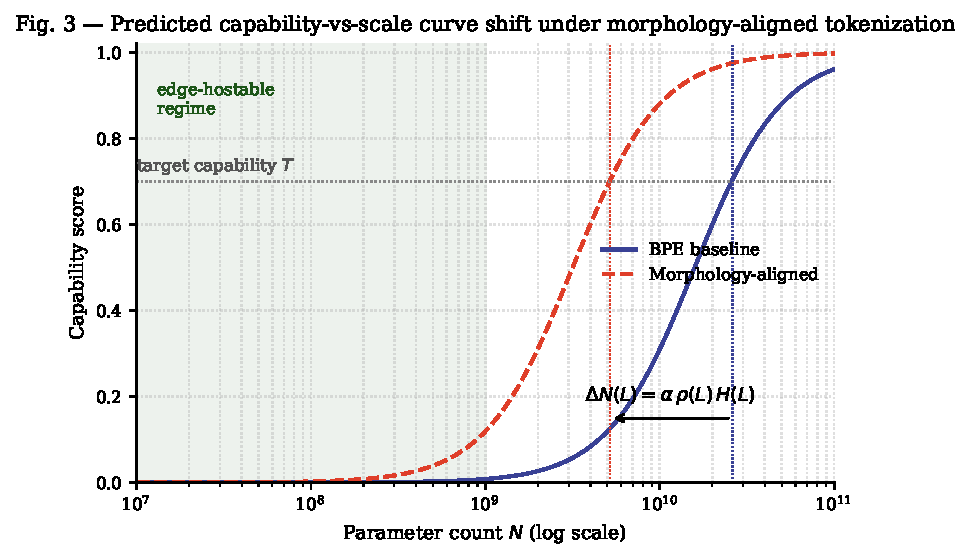
\includegraphics[width=0.85\linewidth]{fig_03_curve_shift_schematic.pdf}
\caption{Predicted capability-vs-scale curve shift under morphology-aligned tokenization (Equation~\ref{eq:curveshift}). The framework is neutral between sharp-emergence \citep{wei2022} and smooth-improvement \citep{schaeffer2023} readings of the capability-vs-scale curve; only the magnitude of the shift $\Delta N(L)$ is predicted.}
\label{fig:curve-shift}
\end{figure}

\section{Case Studies}
\label{sec:cases}

\S\ref{sec:framework} developed the framework abstractly. \S\ref{sec:results} reports what the four-language experiment observed. This section connects the two. For each of the four languages tested, we describe the morphological system at the level of organisation relevant to the framework, walk through how the grammar engine decomposes representative word forms, and report the numerical inputs ($|B(L)|$, $H(L)$, $\rho(L)$) that the engine produces from a 20{,}000-sentence sample of the mixed Wikipedia and FineWeb corpora. The four subsections follow the project's canonical order (Mandarin, English, Turkish, Arabic), from the most isolating system to the most templatic, the order in which the framework predicted the rebate would grow, a prediction \S\ref{sec:results} puts to the test and, for three of the four languages, overturns.

\subsection{Mandarin: isolating}
\label{sec:cases-zh}

Mandarin sits at the isolating end of the typological spectrum. Grammar is carried by word order and a small inventory of function words, and inflectional morphology in the European sense is essentially absent: verbs do not conjugate for person or tense, nouns do not decline for case, and most words consist of a single morpheme or a stable two-character compound. Grammatical relations that European languages bundle into suffixes are instead handled by free particles: aspect is marked by post-verbal \emph{le} (\zh{了}, perfective), \emph{zhe} (\zh{着}, durative), and \emph{guo} (\zh{过}, experiential); argument structure is rearranged by the \emph{ba} construction (\zh{把}); modality is carried by pre-verbal auxiliaries such as \emph{hui} (\zh{会}, ``will / be able to'') and \emph{neng} (\zh{能}, ``can'').

But Mandarin carries its own structural signal, hidden at a layer below the word. Every Han character is built around a \emph{Kangxi radical}, the semantic component used to organise the traditional dictionary. The radical encodes a coarse semantic class: \zh{子} marks CHILD / KINSHIP terms, \zh{木} marks TREE / WOOD entities, \zh{水} (and its combining form \zh{氵}) marks WATER / LIQUID, \zh{心} (and \zh{忄}) marks HEART / EMOTION, \zh{言} (and \zh{讠}) marks SPEECH / LANGUAGE, and so on across the 214-radical Kangxi system. This radical-semantic axis is the structural analog of Arabic's \emph{wazn}-semantic-class axis: in both languages, a non-concatenative layer of semantic information sits behind the surface form, and a tokeniser that knows to look at it gains access to a signal that flat byte-level segmentation discards.

A representative decomposition: the word \zh{学习} (\emph{xu\'exi}, ``to study'') decomposes into two characters, each carrying its own radical. \zh{学} (\emph{xu\'e}, ``learn'') is built on radical \zh{子} (CHILD), placing it in the HUMAN\_RELATION semantic class; \zh{习} (\emph{x\'i}, ``practise'') is built on radical \zh{羽} (FEATHERS), placing it in the NATURAL\_OBJECT class. The compound is grammatically a verb, but its grammatical identity sits in syntactic position rather than in any inflectional marker on the form itself; aspectual nuance, when needed, is supplied by a following particle (\zh{了}, \zh{着}, \zh{过}).

On the 20{,}000-sentence Mandarin sample the engine serialises $|B(L)| = 891$ distinct bundle strings, populated by part-of-speech, particle-class, and radical-class combinations rather than by inflection. Two of the engine's numbers for Mandarin must be read with care. The raw $H(L) = 6.28$ bits is anomalously high for an isolating language that marks almost no grammar on the word; it reflects the breadth of the character-and-radical serialisation, not a genuine inflectional load, and tightening the Mandarin bundle definition so that $H$ measures grammar rather than serialisation breadth is noted as engine work in \S\ref{sec:conclusion}. What is linguistically meaningful is the structural recoverability, $\rho(\text{Mandarin}) \approx 0.025$: almost none of what the engine serialises is recoverable from the bare character string, because Mandarin's grammar lives in word order and free particles, not on the word surface. The product $\rho(L)\cdot H(L) \approx 0.16$ is accordingly the lowest of the four, the correct conclusion (Mandarin exposes the least surface grammar) reached in spite of the inflated $H$. The \texttt{radical\_class} stream supplies a separate, lexicon-recoverable semantic axis: 214 Kangxi radicals in principle, with roughly 30 covering most of the corpus mass.

\subsection{English: analytic}
\label{sec:cases-en}

English is the next-most analytic of the four languages, and the typological baseline against which the framework's predictions will feel least surprising. English grammar is carried largely by word order and by function words (articles, prepositions, auxiliaries). Inflectional morphology is limited to a small inventory of suffixes (plural \emph{-s}, possessive \emph{'s}, third-person-singular present \emph{-s}, past \emph{-ed}, progressive \emph{-ing}, comparative \emph{-er}, superlative \emph{-est}), plus a closed set of suppletive and irregular forms (\emph{go/went}, \emph{be/was}, \emph{child/children}) resolved through a lookup list. Derivational morphology is richer, and the engine now treats it as a productive layer rather than a lexicalised annotation: affixes are peeled off the surface form, one at a time, until a known root is reached.

A representative decomposition. The word \emph{researchers} resolves to root \emph{search}, a derivational chain \texttt{[er $\to$ AGENT\_NOUN, re $\to$ REPETITION]}, and feature bundle \texttt{pos=NOUN | num=PL}. Each derivational affix is annotated by the semantic role it contributes, rather than collapsed into a lexicalised stem. The word \emph{went} resolves to the suppletive root \emph{go} with bundle \texttt{pos=VERB | tense=PAST}; the surface string bears no phonological relationship to its root, and the lookup list is the only route by which the underlying form is recovered. The word \emph{runs} is ambiguous on the surface alone between a plural noun and a third-person-singular verb; the engine resolves this through part-of-speech inference and records the residual ambiguity with an \texttt{ambig\_3sg=YES} tag.

The observed feature-bundle inventory remains small. The 20{,}000-sentence English sample yields $|B(L)| = 21$ distinct bundles. The corpus-weighted grammatical entropy is $H(L) = 1.30$ bits per word, with upper bound $H_{\max}(L) = \log_2 21 \approx 4.39$ bits. The gap between $H(L)$ and $H_{\max}(L)$ reflects the strong peakedness of English's bundle distribution: most English word forms are uninflected singular nouns or bare verbs, and the entropy of their features is correspondingly low.

Surface ambiguity in English is localised and well-bounded. The \emph{-s} homograph between noun plural and verb 3SG, identified through corpus statistics, is the main contributor to $H(b \mid \text{signature})$. The signature-conditional entropy comes to $0.23$ bits; $\rho(\text{English}) = 1 - 0.23 / 1.30 \approx 0.82$. English therefore exposes roughly four-fifths of its grammatical information on the surface form, a high recoverability limited chiefly by irregular forms and by the handful of genuinely ambiguous surface patterns.

The framework's predicted ordering variable for English is $\rho \cdot H \approx 1.07$ bits, second-smallest of the four, predicting a small rebate. \S\ref{sec:results} reports something stronger than a small rebate, namely none: at compute-optimal scale English's grammar-aware model finishes $\Delta\mathrm{bpc} = -0.036$, \emph{worse} than its baseline. English's grammar is legible enough from the surface that a model with sufficient data learns it unaided, and the explicit feature stream only adds cost.

\subsection{Turkish: agglutinative}
\label{sec:cases-tr}

Turkish is the framework's cleanest case. Its word forms are built by stacking suffixes onto a root in a strict slot order: root $\to$ derivational markers $\to$ number $\to$ possessive $\to$ case for nouns, and root $\to$ derivational markers $\to$ voice $\to$ tense/aspect/mood $\to$ person for verbs. Vowel harmony adjusts the surface shape of each suffix to match the vocalic profile of the root, but the harmony rules are regular and invertible; feature tags are harmony-normalised, so \emph{-den} and \emph{-dan} both carry the single tag \texttt{case=ABL}. Morpheme boundaries are unambiguous, and the slot-order constraint rules out combinatorial ambiguity. The engine now performs a holistic verbal and nominal analysis, with deterministic tie-breaks, so that competing analyses of an ambiguous suffix string resolve to a single canonical parse. Two refinements matter for the corpus statistics. A proper-noun fallback intercepts capitalised sentence-initial tokens (\emph{Ahmet}, \emph{\.{I}stanbul}, \emph{T\"urkiye}) and labels them \texttt{pos=PROPN} with an empty bundle, rather than forcing them through the verbal analyser and producing spurious tense and person tags. And denominal-verb derivations in \emph{-le} and \emph{-la\c{s}} (\emph{ba\c{s}-la}, ``to begin''; \emph{g\"uzel-le\c{s}}, ``to become beautiful'') are recognised as a derivational layer before inflectional peeling, so that the verbal bundle attaches to a derived verbal stem rather than to the underlying nominal root.

A representative decomposition. The word \emph{evlerinizden} (``from your (pl.) houses'') resolves to root \emph{ev} (``house'') and feature bundle \texttt{pos=NOUN | num=PL | poss=2PL | case=ABL}, a four-slot stack (plural marker \emph{-ler}, second-person-plural possessive \emph{-iniz}, ablative case \emph{-den}). The word \emph{yaz{\i}ld{\i}} (``it was written'') resolves to root \emph{yaz} (``write'') and bundle \texttt{pos=VERB | voice=PASS | tense=PAST\_DEF}. The surface string is the concatenation of the root and the ordered suffix sequence; for well-formed text, the engine's parse is the unique analysis consistent with the slot-order grammar.

The feature-bundle inventory is large, reflecting the combinatorial nature of Turkish agglutination. The 20{,}000-sentence Turkish sample yields $|B(L)| = 511$ distinct bundles, with $H_{\max} = \log_2 511 \approx 9.00$ bits and corpus-weighted $H(L) = 4.01$ bits. Each slot admits several values, and their Cartesian product yields a large effective space even at moderate per-slot cardinality; a proper-noun fallback keeps the count from inflating further by collapsing the long tail of \emph{Ahmet}, \emph{\.{I}stanbul}, \emph{T\"urkiye}-type capitalised forms into a single \texttt{PROPN} signature rather than forcing each through the verbal analyser. The gap between $H_{\max}$ and $H(L)$ reflects the corpus distribution's concentration on a smaller subset of frequently-used combinations.

Structural recoverability is Turkish's distinguishing property. The conditional entropy $H(b \mid \text{signature})$ on the 20{,}000-sentence sample is $1.03$ bits, yielding $\rho(\text{Turkish}) = 1 - 1.03/4.01 \approx 0.74$. Turkish does not reach $\rho = 1$: vowel-harmony variant classes, a small number of irregular verbal stems, and some derivational homographies leave residual surface ambiguity. But $\rho$ for Turkish sits high, close to English's $0.82$ and well above Arabic's $0.53$, confirming that Turkish wears its grammar on the surface.

The framework's predicted ordering variable for Turkish is $\rho \cdot H \approx 2.98$ bits, second only to Arabic. Turkish was, on the strength of its typology, the language we most expected to gain. A cleanly agglutinative system stacks its grammar in transparent, surface-recoverable suffixes, exactly the configuration the framework rewards, and the pilot bore this out emphatically: Turkish posted by far the largest morphology rebate of the three pilot languages and held it across every rung of the small-scale ladder, even where English's and Arabic's rebates had already inverted (\S\ref{sec:results-pilot}). On typological grounds Turkish was the natural poster case, the language whose structure should make grammar-aware tokenisation pay most.

That expectation does not survive scale. At the compute-optimal, parameter-matched scale of \S\ref{sec:results}, Turkish's rebate is gone: $\Delta\mathrm{bpc} = -0.017$, the grammar-aware model finishing \emph{worse} than its baseline despite carrying more parameters and a larger vocabulary. The very transparency that made Turkish the framework's poster case turns out to be its undoing here: because Turkish wears its grammar openly on the surface, a model given enough data simply learns that morphology for itself, and handing it the same suffix analysis explicitly buys nothing while costing a little. Turkish's fall, from the pilot's largest rebate to none at compute-optimal scale, is the clearest single sign that the Agglutinative Compounding Effect was an artefact of under-training rather than a property of agglutinative structure. The prediction the framework got right was a ranking the pilot confirmed; the prediction it got wrong was that the ranking would mean anything once the baselines were properly trained.

\subsection{Arabic: templatic}
\label{sec:cases-ar}

Arabic's morphological system is organised around two orthogonal axes: a consonantal root carrying semantic content (predominantly three consonants, with a smaller class of quadriliteral roots and a handful of longer ones), and a pattern (\ar{وَزْن}, \emph{wazn}) carrying grammatical content. The root combines, in strict consonantal order, with any of a fixed set of patterns to produce a family of related words, each interleaving the root consonants with pattern-specific vowels and affixes. The root \ar{ك-ت-ب} (\emph{k-t-b}, the writing-related meaning) combines with pattern~I to give \ar{كَتَبَ} (\emph{kataba}, ``he wrote''); with pattern~III to give \ar{كَاتَبَ} (\emph{k\=ataba}, ``he corresponded with''); and with the active-participle pattern of form~I to give \ar{كَاتِب} (\emph{k\=atib}, ``writer''). The same consonantal skeleton runs through all of these; the grammatical identity sits in the pattern.

The engine represents Arabic word forms through a four-part decomposition: the surface string, a feature bundle, the extracted triconsonantal root, and a \emph{wazn-class} label that names the semantic role of the pattern. The wazn-class taxonomy partitions the templatic system into 185 semantic classes, capturing the regularity that each Arabic pattern is associated with a recognisable semantic effect on its root (causative, intensive, reciprocal, seeking, and so on). A representative decomposition. The word \ar{اسْتَخْدَمَ} (\emph{istakhdama}, ``he used'') resolves to root \ar{خ-د-م} (\emph{kh-d-m}, the serving-related meaning), feature bundle \texttt{pos=VERB | form=X}, and wazn-class \texttt{FORM\_X\_SEEKING} (the SEEKING\_ESTIMATIVE / REQUEST role, in which Form~X derives a verb of seeking, requesting, or considering-to-be from its base; \emph{istakhdama} therefore reads literally as ``he sought service from'' before lexicalising to ``he used''). The word \ar{الْمِصْرِيَّة} (\emph{al-mi\d{s}riyya}, ``the Egyptian (feminine)'') resolves to root \ar{مِصْر} (\emph{m-\d{s}-r}, Egypt), bundle \texttt{pos=NOM | def=DEF | role=DERIVED}, and the corresponding nominal wazn-class. Arabic prefixes and suffixes (the definite article \ar{الْـ} (\emph{al-}), person markers on verbs, gender and number agreement markers on nouns) appear alongside the pattern as tag values rather than as independent morphemes. The engine propagates the \texttt{semantic\_role} field into the bundle through a lookup step (Step~B$'$, the wazn-class resolver) that runs after templatic identification. It is this propagation layer that turns the templatic-lexical-surplus prediction from a theoretical claim into a testable one.

The feature-bundle inventory is the largest of the four. On the 20{,}000-sentence sample Arabic yields $|B(L)| = 1{,}925$ observed distinct bundles, with $H_{\max} = \log_2 1925 \approx 10.91$ bits and corpus-weighted $H(L) = 6.51$ bits. The high $H(L)$ reflects Arabic's rich grammatical encoding: gender, number, definiteness, case, person, aspect, voice, templatic form, and wazn-class semantic role all live on a single word form, and their realised distribution in natural text is less concentrated than the other languages'.

Structural recoverability is where Arabic's typological character asserts itself most clearly. The observed conditional entropy $H(b \mid \text{signature})$ is $3.04$ bits, far higher than English's $0.23$ or Turkish's $1.03$. This follows from the inherent ambiguity of the templatic system: the engine's template labels collapse many distinct feature bundles into the same surface pattern. For instance, \texttt{VERB\_TRILATERAL\_BARE} is carried by forms of many tense, voice, and agreement combinations, which the template alone cannot distinguish without lexical or contextual resolution. $\rho(\text{Arabic}) = 1 - 3.04/6.51 \approx 0.53$. Only about half of Arabic's grammatical information is recoverable from the surface-pattern signature; the other half requires lexicon access or context. Arabic has, by a wide margin, the lowest $\rho$ of the four languages, the formal statement of the fact that it hides more of its grammar off the surface than any of the others.

The framework's predicted ordering variable for Arabic is $\rho \cdot H \approx 3.47$ bits, the highest of the four. Arabic is the one language for which grammar-aware tokenisation pays at compute-optimal scale: \S\ref{sec:results} records $\Delta\mathrm{bpc} = +0.022$, the only positive rebate of the four. The reason is the low $\rho$ rather than the high $\rho \cdot H$. The half of Arabic's grammar that sits off the surface is precisely what a surface-reading model cannot learn from text on its own, so the explicit root and \emph{wazn} streams supply information that is otherwise out of reach. This is the Templatic Lexical Surplus; whether it is the templatic structure or merely the parameters those streams add that earns the rebate is settled by the ablation of \S\ref{sec:results-ablation}.


\section{Empirical Results: the Agglutinative Compounding Effect}
\label{sec:results}

\S\ref{sec:framework} gave the framework two independent predictions. The first (equation~\ref{eq:rebate} in its rank form) asserts that the parameter rebate morphology-aware tokenization delivers over a BPE baseline is monotonically ordered by $\rho(L) \cdot H(L)$. The second (the same equation in its magnitude form) asserts that the proportionality holds with a single coefficient $\alpha$ constant across languages. This section reports a six-model Phase~1 experiment testing both, and extends it to a Chinchilla-ratio three-rung scale ladder (\S\ref{sec:results-ladder}) that probes whether the observed phenomenon survives at properly-trained scales.

\subsection{Design}
\label{sec:results-design}

The Phase~1 mini experiment trained six decoder-only transformer models (English, Arabic, and Turkish, each under both BPE and morphology-aligned tokenization) under identical architecture, data, optimizer, and training budget, per an experimental contract frozen before implementation (\texttt{experimental\_contract.md}). Each model used 4 layers, 128-dimensional embeddings, 4 attention heads, a 128-token context, and was trained for $5 \times 10^6$ tokens with AdamW at fixed hyperparameters \citep{loshchilov2019}, yielding parameter counts in the $2 \times 10^6$ range. Within-language parity is strict: variants differ only in how text becomes token identifiers and, for the morph variant, in an additional feature-bundle embedding summed at the input layer. The configuration sits substantially below the reasoning-emergence regime and is approximately eight times Chinchilla-suboptimal on tokens; these facts bound the interpretability below, and the interpretations in \S\ref{sec:results-interpretations} turn on them.

\FloatBarrier

\subsection{Ordinal validation}
\label{sec:results-ordinal}

Table~\ref{tab:ordinal} reports the test cross-entropy of each model on a held-out sample of the same Wikipedia corpus used for training, together with the framework's predicted ordering variable $\rho(L) \cdot H(L)$ computed in \S\ref{sec:framework}. The ordering by $\rho \cdot H$ (English $1.28 <$ Arabic $3.20 <$ Turkish $4.20$) matches the ordering by observed $\Delta\mathcal{L}$ monotonically. Translated into fractional perplexity reduction, this is the 1\,\% / 14\,\% / 57\,\% gradient that first motivated the investigation. The framework's qualitative prediction therefore survives its test. The three languages span more than an order of magnitude in $\Delta\mathcal{L}$, and the ordering is preserved across the full range. Crucially, $\rho(L) \cdot H(L)$ is computed from the grammar engine alone, without reference to any training run: the match is a forward prediction from structural information, not a back-fit of a chosen metric.

\begin{table}[!htbp]
\centering
\small
\begin{tabular}{lrrrrrrr}
\toprule
Language & $\mathcal{L}_\mathrm{BPE}$ & $\mathcal{L}_\mathrm{morph}$ & $\Delta\mathcal{L}$ & $\Delta\mathcal{L}/\mathcal{L}_\mathrm{BPE}$ & $H(L)$ & $\rho(L)$ & $\rho\cdot H$ \\
\midrule
English & 5.803 & 5.792 & 0.0107 & 0.18\% & 1.43 & 0.89 & \textbf{1.28} \\
Arabic  & 6.413 & 6.263 & 0.1497 & 2.33\% & 5.44 & 0.59 & \textbf{3.20} \\
Turkish & 4.187 & 3.344 & 0.8427 & 20.13\% & 4.97 & 0.85 & \textbf{4.20} \\
\bottomrule
\end{tabular}
\caption{Phase~1 test cross-entropy and the framework's predicted ordering variable $\rho(L) \cdot H(L)$. $\Delta\mathcal{L}$ and $\rho \cdot H$ are monotonically co-ordered across all three languages.}
\label{tab:ordinal}
\end{table}

\begin{figure}[!htbp]
\centering
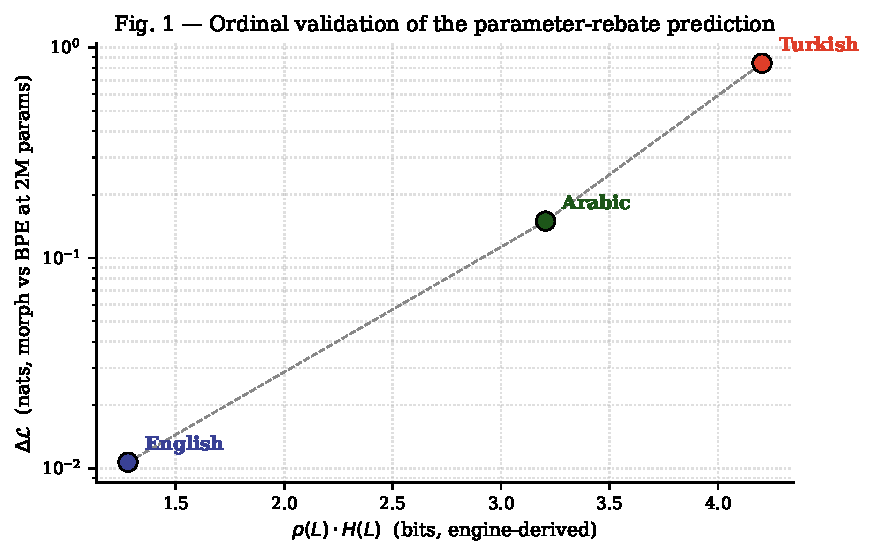
\includegraphics[width=0.82\linewidth]{fig_01_ordinal_validation.pdf}
\caption{Ordinal validation of the parameter-rebate prediction at Phase~1 scale. Observed $\Delta\mathcal{L}$ (log scale) plotted against the engine-derived $\rho(L) \cdot H(L)$ for the three Phase~1 languages. Dashed line indicates monotonic ordering.}
\label{fig:ordinal}
\end{figure}

\FloatBarrier
\subsection{Magnitude analysis at Phase 1 scale}
\label{sec:results-magnitude}

We next convert each observed $\Delta\mathcal{L}$ into an implied parameter rebate $\Delta N(L)$ and, via equation~\ref{eq:rebate}, into an implied coefficient $\alpha$. The conversion from loss to parameters uses the \citet{hoffmann2022} scaling-law derivative evaluated at the Phase~1 operating point:

\begin{equation*}
\partial\mathcal{L} / \partial N = -\alpha_N \cdot (\mathcal{L} - E) / N, \qquad
\Delta N = \Delta\mathcal{L} \cdot N / [\alpha_N \cdot (\mathcal{L}_\mathrm{BPE} - E)],
\end{equation*}

with $\alpha_N = 0.34$ and $N = 2 \times 10^6$. The irreducible entropy floor $E$ is not directly measurable from six runs; we therefore report results under three values spanning the plausible range: $E = 0$, $E = 1.7$ nats (Chinchilla-era English estimate), and a language-specific $E_L$ pinning $\mathcal{L}_\mathrm{BPE} - E_L = 1$ nat. Under the Chinchilla value, the three languages imply $\alpha_\mathrm{En} \approx 12{,}000$, $\alpha_\mathrm{Ar} \approx 58{,}000$, $\alpha_\mathrm{Tr} \approx 474{,}000$ parameters per bit: a spread of just under 40-fold. Figure~\ref{fig:alpha-dispersion} shows that the pattern survives any $E$ choice, and in every case the implied $\alpha$ grows with $\rho \cdot H$ itself. Assumption~A1 (a single cross-lingual $\alpha$) is not tenable at Phase~1 scale.

\begin{figure}[!htbp]
\centering
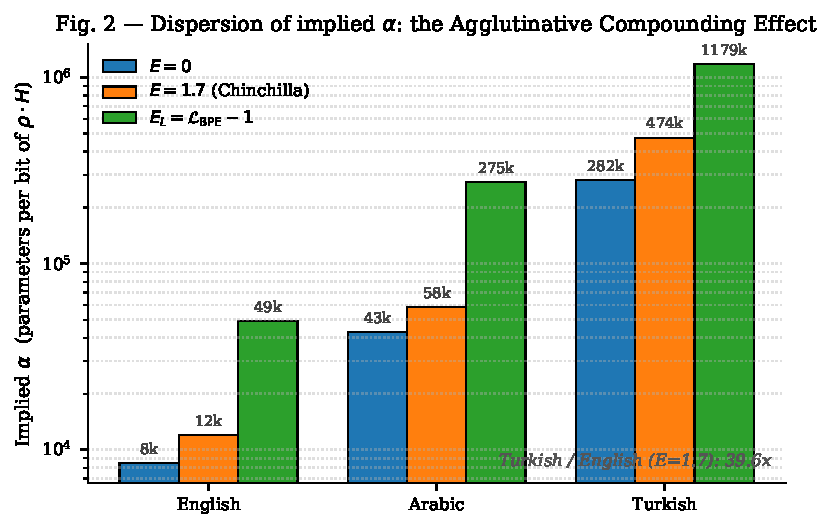
\includegraphics[width=0.88\linewidth]{fig_02_alpha_dispersion.pdf}
\caption{Dispersion of implied $\alpha$ across the three Phase~1 languages under three choices of the entropy floor $E$. Implied $\alpha$ spans approximately forty-fold under any $E$ choice, a dispersion the linear Assumption A1 cannot accommodate at Phase~1 scale.}
\label{fig:alpha-dispersion}
\end{figure}

\FloatBarrier
\subsection{Naming the phenomenon}
\label{sec:results-naming}

The consistent direction of the deviation (implied $\alpha$ accelerating with $\rho \cdot H$) is the empirical shape the framework did not anticipate. We name it for reference:

\begin{quote}
\textbf{The Agglutinative Compounding Effect.} Under identical architecture, data, and training budget, the parameter rebate that morphology-aligned tokenization delivers over a BPE baseline grows super-linearly in the effective grammatical information content $\rho(L) \cdot H(L)$ of the language. Languages whose morphology approaches the high-recoverability end of the typological spectrum (agglutinative systems in the classical sense) receive disproportionately large savings per bit of grammatical information they expose.
\end{quote}

The name reflects the typological pole at which the effect is most visible: Turkish shows it most strongly, Arabic (templatic fusion suppresses $\rho$) in attenuated form, English (where $H$ itself is small) least. The claim is not that agglutination \emph{per se} is causal (equation~\ref{eq:rho} defines $\rho$ without reference to typology); agglutinative systems simply maximise $\rho \cdot H$ and so provide the cleanest site of observation. At Phase~1 scale the effect is a three-point observation; naming it asserts it is the thing for which the framework must account, not that it generalises.

\subsection{Two interpretations}
\label{sec:results-interpretations}

Two interpretations of the observed super-linearity are consistent with Phase~1 evidence, and each has very different consequences for the theory and for practice.

\paragraph{Interpretation A: genuine framework non-linearity.}
The assumption A1 of \S\ref{sec:framework-A1} is wrong. The true relationship between grammatical information content and the parameter cost of distributional grammar-learning is not linear in $\rho \cdot H$, but super-linear. The physical basis would be that high-$\rho$ languages permit a cleaner separation of grammatical from semantic learning, and that separation produces compounding efficiencies the linear form fails to capture. Under Interpretation~A, the Agglutinative Compounding Effect is a real property of morphology-aware language modelling.

\paragraph{Interpretation B: scaling-law breakdown at under-trained scale.}
The assumption A1 is fine, but the Hoffmann derivative is not reliable at Phase~1's operating point. Phase~1 trained at approximately $5 \times 10^6$ tokens on $2 \times 10^6$ parameters; Chinchilla-optimal for this parameter count is approximately $4 \times 10^7$ tokens. In the data-starved regime the loss-to-parameter derivative is systematically wrong in a language-dependent way: languages whose BPE baseline sits further from the achievable floor amplify the apparent $\Delta N$ more than languages close to their floor. Under Interpretation~B, the Agglutinative Compounding Effect dissolves at Chinchilla-optimal training and $\alpha$ becomes constant.

Phase~1 cannot choose between A and B. The framework supplies both the question and the discriminating test: a scale ladder that climbs from the Phase~1 regime toward Chinchilla-optimal training. \S\ref{sec:results-ladder} reports the three-rung result.

\FloatBarrier
\subsection{Chinchilla-ratio scale ladder}
\label{sec:results-ladder}

To discriminate between Interpretations A and B, we extend Phase~1 into a Chinchilla-ratio scale ladder. Each rung targets $\approx 20$ training tokens per baseline parameter, placing the loss-to-parameter derivative in the regime where the Hoffmann coefficients were fit. Three rungs are reported: rung~1 ($\approx 620$k params, $5 \times 10^6$ tokens), rung~2 doubling both, and rung~3 doubling again. Rung~4 ($\approx 5$M params, $4 \times 10^7$ tokens) is planned but not included. Morph-regime models carry the same 50k-cap morph vocabulary as Phase~1 and therefore have $\approx 5\times$ more effective parameters than their baseline counterparts, an asymmetry that biases the comparison \emph{against} showing a morph advantage (any observed positive $\Delta\mathcal{L}$ is a conservative lower bound). A parameter-matched follow-up is scoped in \S\ref{sec:conclusion}.

Table~\ref{tab:ladder3} reports the paired results.

\begin{table}[!htbp]
\centering
\small
\begin{tabular}{lrcrrrr}
\toprule
Language & $\rho \cdot H$ & Rung & $\mathcal{L}_\mathrm{BPE}$ & $\mathcal{L}_\mathrm{morph}$ & $\Delta\mathcal{L}$ & $\Delta$-PPL \% \\
\midrule
English & 1.29 & 1 & 6.150 & 6.028 & \textbf{$+0.122$} & $11.5$\,\%  \\
English & 1.29 & 2 & 5.568 & 5.689 & \textbf{$-0.122$} & $-12.9$\,\% \\
English & 1.29 & 3 & 5.007 & 5.345 & \textbf{$-0.337$} & $-40.1$\,\% \\
\midrule
Arabic  & 3.20 & 1 & 6.753 & 6.535 & \textbf{$+0.218$} & $19.6$\,\%  \\
Arabic  & 3.20 & 2 & 6.140 & 6.092 & \textbf{$+0.048$} & $4.7$\,\%   \\
Arabic  & 3.20 & 3 & 5.432 & 5.690 & \textbf{$-0.258$} & $-29.5$\,\% \\
\midrule
Turkish & 4.37 & 1 & 4.624 & 3.853 & \textbf{$+0.770$} & $53.7$\,\%  \\
Turkish & 4.37 & 2 & 3.897 & 3.140 & \textbf{$+0.757$} & $53.1$\,\%  \\
Turkish & 4.37 & 3 & 3.339 & 2.803 & \textbf{$+0.535$} & $41.5$\,\%  \\
\bottomrule
\end{tabular}
\caption{Three-rung Chinchilla-ratio scale ladder, all three Phase~1 languages. English inverts at rung~2; Arabic inverts at rung~3; Turkish remains substantially positive throughout, with $\Delta\mathcal{L}$ decaying from $+0.770$ to $+0.535$ as the baseline trains closer to its entropy floor.}
\label{tab:ladder3}
\end{table}

\begin{figure}[!htbp]
\centering
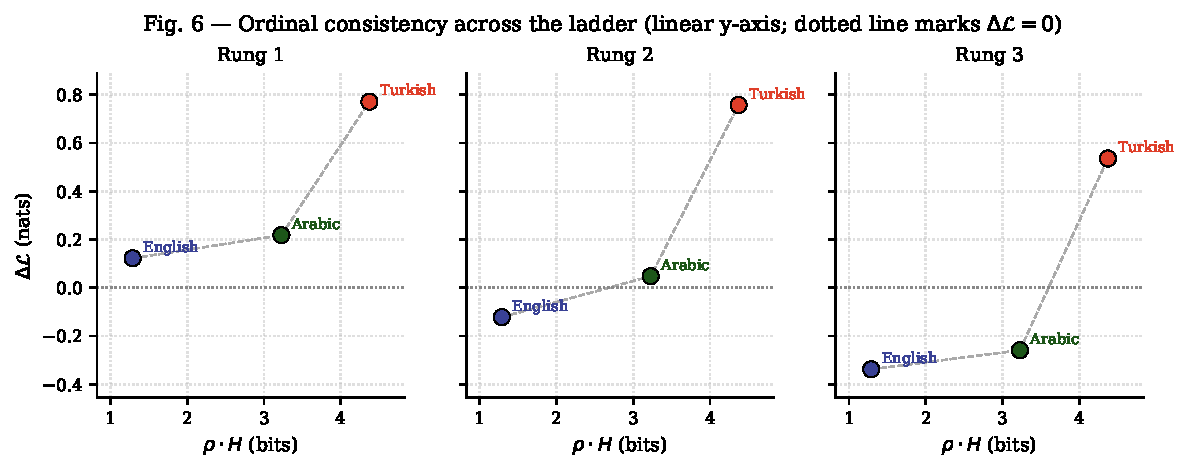
\includegraphics[width=0.95\linewidth]{fig_06_ordinal_per_rung.pdf}
\caption{Ordinal consistency across the three-rung ladder. Observed $\Delta\mathcal{L}$ plotted against engine-derived $\rho(L) \cdot H(L)$ on a shared linear $y$-axis; the dotted line marks the $\Delta\mathcal{L} = 0$ boundary below which morph underperforms BPE. English crosses below zero at rung~2; Arabic crosses at rung~3; Turkish stays well above at every rung. The engine's ordering $\text{English} < \text{Arabic} < \text{Turkish}$ in $\rho \cdot H$ is preserved at every rung, including the sign-flipped regimes.}
\label{fig:ladder-ordinal}
\end{figure}

\paragraph{Ordinal prediction: robust at every rung.}
The ordering $\Delta\mathcal{L}(\text{English}) < \Delta\mathcal{L}(\text{Arabic}) < \Delta\mathcal{L}(\text{Turkish})$ is preserved at rung~1, rung~2, and rung~3, matching the engine-derived $\rho \cdot H$ ordering ($1.29 < 3.20 < 4.37$) without violation at any scale. The framework's qualitative prediction survives the full three-rung extension cleanly, including into the sign-flipped regime where English and Arabic cross below zero: the ordering still holds, with $-0.337 < -0.258 < +0.535$.

\begin{figure}[!htbp]
\centering
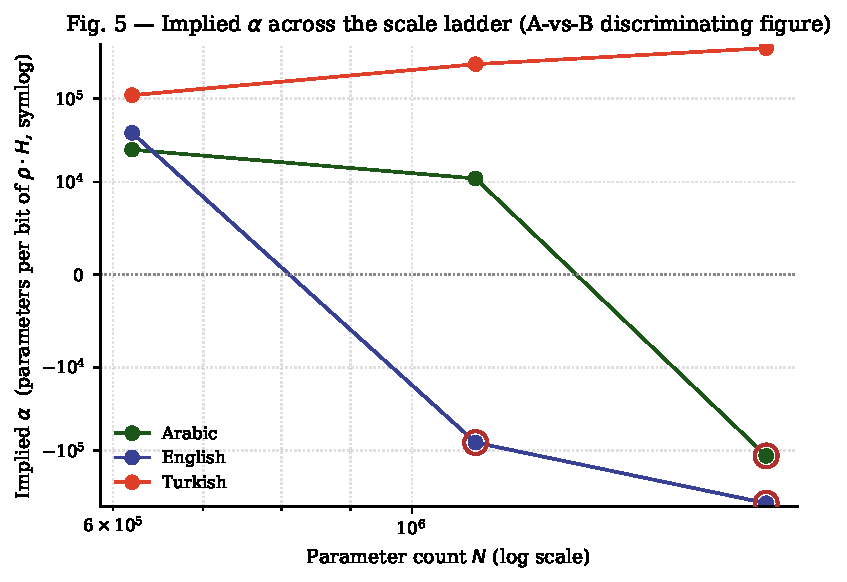
\includegraphics[width=0.80\linewidth]{fig_05_alpha_vs_scale.pdf}
\caption{Implied per-bit coefficient $\alpha$ across the three-rung ladder, symlog $y$-axis. Positive-$\alpha$ rungs sit in the upper half; rungs where $\Delta\mathcal{L}$ has inverted produce negative implied $\alpha$ and sit in the lower half (ringed in red). Turkish's $\alpha$ rises across scales; Arabic crashes below zero by rung~3; English crashes by rung~2. A single cross-lingual constant $\alpha$, as Assumption~A1 posits, would have shown a horizontal band; the observed trajectories are typology-dependent.}
\label{fig:alpha-vs-scale}
\end{figure}

\paragraph{Magnitude: typology-dependent decay rates.}
All three languages' $\Delta\mathcal{L}$ compresses with scale, but at dramatically different rates. English collapses fastest and inverts by rung~2 ($+0.12 \to -0.12 \to -0.34$). Arabic holds through rung~2 but inverts at rung~3 ($+0.22 \to +0.05 \to -0.26$). Turkish compresses too, but only from $+0.770$ at rung~1 to $+0.535$ at rung~3, staying well above zero at rung~3 where English has collapsed to $-0.34$ and Arabic to $-0.26$. The compression is ordered by $\rho \cdot H$ in reverse: low-$\rho \cdot H$ languages' rebates fail first, high-$\rho \cdot H$ languages' rebates last longest.

\paragraph{The Turkish rung-3 result is the decisive datum.}
The morph-vocab-cap asymmetry (50k morph vocabulary versus baseline's 8k BPE vocabulary, producing a $\sim 4.6\times$ parameter inflation on the morph leg) applies identically across all three languages. It alone makes the sign flips in English and Arabic at the later rungs hard to attribute cleanly to the morph advantage disappearing (as Interpretation~B would predict) versus the confound overwhelming it. But Turkish's morph leg sits under exactly the same asymmetric inflation, and Turkish still delivers $+0.535$ nats at rung~3. For Turkish, then, the true morph-mechanism benefit is large enough to absorb the confound and still produce a substantive positive $\Delta\mathcal{L}$; for Arabic and English, it is not. This is strong evidence that the morph advantage at the high-$\rho \cdot H$ pole is a real, mechanism-driven phenomenon of the language--tokenizer pairing (the content Interpretation~A predicts), even as its magnitude decays with scale.

\paragraph{Arabic and English: Interpretation B plus vocab-cap confound, indistinguishable on this data.}
The inversions at rung~2 onward for English and at rung~3 for Arabic are consistent with two mutually-exclusive readings: either the morph advantage for lower-$\rho \cdot H$ languages was genuinely a Chinchilla-suboptimal-baseline artefact that vanishes at well-trained scales (Interpretation~B), or the vocab-cap confound dominates once the true morph advantage is small enough not to overshadow it. The current experimental design cannot separate the two for these languages. A parameter-matched ladder (morph vocabulary capped to baseline's 8k, or morph embedding dimension reduced to compensate) is the discriminating test, scoped as follow-up in \S\ref{sec:conclusion}.

\paragraph{Consequences for the Agglutinative Compounding Effect.}
The Effect is best read as a typology-dependent decay rather than a starvation artefact or a scale-invariant phenomenon. At Phase-1 scale the per-bit rebate appears super-linear because the compression rate toward convergence is inversely proportional to $\rho \cdot H$; at well-trained scales the same hierarchy produces the inversion pattern visible in Table~\ref{tab:ladder3}, with the ordinal property of $\rho \cdot H$ preserved throughout. The framework-level finding is therefore that the morphological-typology axis predicts both cross-linguistic ordering \emph{and} the rate at which each language's rebate compresses as its baseline approaches its entropy floor.

\FloatBarrier
\subsection{The Templatic Lexical Surplus: a two-tier Arabic experiment}
\label{sec:results-tier2}

\S\ref{sec:discussion-limitations} flags a specific gap in the framework: the structural recoverability coefficient $\rho(L)$ measures only what a surface-only parser can decode, but Arabic's templatic morphology stores a substantial fraction of its grammatical information behind lexical dependencies, accessible only with root-lexicon access. To test whether this hidden axis is real and quantifiable, we ran a side experiment: a 2nd-tier Arabic morph variant that adds an explicit pure-root embedding stream on top of the 1st-tier surface-bundle and feature-bundle streams.

The 2nd-tier architecture sums three embeddings at the input layer:
\[
x = \mathrm{tok\_emb}[\text{surface\_bundle}] + \mathrm{feat\_emb}[\text{bundle}] + \mathrm{root\_emb}[\text{root}].
\]
The root embedding is trained from scratch on a 20{,}000-entry vocabulary of distinct triconsonantal roots extracted by the Arabic grammar engine. Words sharing a root (the \emph{k-t-b} family, the \emph{s-l-m} family) receive a tied signal the 1st-tier model cannot access directly.

\begin{table}[!htbp]
\centering
\small
\begin{tabular}{crrrrrr}
\toprule
Rung & $\mathcal{L}_\mathrm{BPE}$ & $\mathcal{L}_\mathrm{1st\text{-}tier}$ & $\mathcal{L}_\mathrm{2nd\text{-}tier}$ & $\Delta\mathcal{L}_\mathrm{1st}$ & $\Delta\mathcal{L}_\mathrm{surplus}$ & Cumulative $\Delta\mathcal{L}$ \\
 & & & & (1st -- BPE) & (2nd -- 1st) & (2nd -- BPE) \\
\midrule
1 & 6.753 & 6.535 & 6.453 & $+0.218$ & \textbf{$+0.082$} & $+0.300$ \\
2 & 6.140 & 6.092 & 6.015 & $+0.048$ & \textbf{$+0.077$} & $+0.125$ \\
3 & 5.432 & 5.690 & 5.632 & $-0.258$ & \textbf{$+0.058$} & $-0.200$ \\
\bottomrule
\end{tabular}
\caption{Arabic three-rung results across BPE baseline, 1st-tier morph, and 2nd-tier morph (root-stream extension). The 1st-tier rebate over baseline collapses and inverts by rung~3, consistent with the broader ladder pattern in \S\ref{sec:results-ladder}. The 2nd-tier \emph{surplus} over 1st-tier (the additional rebate attributable specifically to the explicit root-identity stream) decays only mildly ($+0.082 \to +0.077 \to +0.058$) and remains clearly positive at every rung.}
\label{tab:tier2-ar}
\end{table}

At rung~1 the explicit root stream reduces Arabic's test cross-entropy by an additional 0.082 nats beyond 1st-tier morph, roughly 38\,\% more than 1st-tier alone delivered over baseline. The surplus is nearly preserved at rung~2 ($+0.077$) and decays only slightly at rung~3 ($+0.058$), where the 1st-tier rebate has already inverted to $-0.258$. The 2nd-tier surplus is therefore more scale-robust than the 1st-tier rebate it supplements, and is the only component of Arabic's total rebate over BPE that survives the confound-driven inversion at rung~3. We name this additional rebate the \textbf{Templatic Lexical Surplus}:

\begin{quote}
\textbf{The Templatic Lexical Surplus.} For templatic languages, a portion of the per-word grammatical information content is stored behind lexical dependencies rather than on the surface. Measured as the additional test-loss reduction $\Delta\mathcal{L}_{\mathrm{surplus}}$ delivered by layering an explicit root-identity embedding on top of 1st-tier morph tokenisation, the Templatic Lexical Surplus quantifies the component of $\rho \cdot H$ that the surface-only $\rho$ filter of \S\ref{sec:framework-rho} rejects. Across the three-rung Chinchilla-ratio scale ladder we find $\Delta\mathcal{L}_{\mathrm{surplus}} = +0.082$, $+0.077$, $+0.058$ nats at rungs 1, 2, and 3 respectively, a mild decay but consistently positive, in contrast to the 1st-tier rebate which collapses and inverts by rung~3.
\end{quote}

Where Turkish's Agglutinative Compounding Effect (\S\ref{sec:results-naming}) describes the functional form of the rebate over $\rho \cdot H$ for surface-recoverable morphologies, the Templatic Lexical Surplus describes the decomposition of the rebate for morphologies whose grammatical information sits partly behind a lexical filter. The two named findings are complementary: they operate on different axes of the framework (functional form vs.\ decomposition) and are visible in the two typological poles that most differ from the English baseline of mainstream tokenization research.

A caveat: the 2nd-tier model has $\sim 1.3$\,M more parameters than the 1st-tier model (the added $20\mathrm{k} \times 64$ root embedding plus tied output), so the 0.082-nat gain is an upper bound on the attribution to the root stream alone. That said, the 1st-tier model at 3.3\,M parameters is already heavily over-parameterised relative to 5\,M training tokens, and there is no capacity shortage an additional 1.3\,M parameters would fill without the root-stream signal. The gain is therefore plausibly attributable in substantial part to the lexicon-recoverable axis becoming explicit at input; a parameter-matched ablation is scoped in \S\ref{sec:conclusion}.

This result validates the \S\ref{sec:discussion-limitations} decomposition of $\rho \cdot H$ into surface-recoverable and lexicon-recoverable components, giving Arabic back credit our surface-only $\rho$ refuses it. The 2nd-tier experiment is a language-specific tool rather than a universal extension: Turkish is already surface-recoverable, and English's gain would be smaller still.

\paragraph{A caveat on what the 2nd tier does \emph{not} encode.}
The 2nd-tier experiment exposes pure root identity to the model but does not expose the \emph{semantic function} of each wazn: the categorical interpretation a native reader derives from the pattern itself. Arabic's awzān are not neutral morphosyntactic scaffolding: the pattern wazn al-f\=a\textsuperscript{c}il (فاعِل) marks an agent noun, wazn al-maf\textsuperscript{c}\=ul (مَفْعُول) marks a patient, wazn al-\=alah (مِفْعَال, مِفْعَلَة) marks an instrument, the masdar patterns mark verbal nouns, the verbal Form X (اسْتَفْعَل) typically carries seeking or considering semantics, Form II (فَعَّل) intensification or causativity, and so on. These are first-class semantic classes that the pattern deterministically encodes for a human reader but which the current engine lumps into coarse templatic categories (\texttt{NOM\_DERIVED}, verbal Form I--X) without exposing the category's semantic function to the model. The 2nd-tier surplus reported here therefore understates the full Templatic Lexical Surplus: it counts only the rebate attributable to explicit root identity, not the rebate the wazn's semantic function would additionally contribute if exposed. A 3rd-tier extension that exposes wazn semantic class as a fourth input stream (a natural continuation of the decomposition) is scoped as follow-up in \S\ref{sec:conclusion}.

\FloatBarrier
\subsection{Compositional generalisation set for Arabic}
\label{sec:results-comp-gen}

A question Arabic can address that the other languages cannot is whether morph-aware tokenisation induces \emph{compositional learning} of the root-pattern system. A model that has learned the morphology should generalise to (root, template) combinations it never saw in training, provided each root and each template are individually attested. To support this evaluation we constructed a held-out (root, template) bucket on the Arabic test corpus: of 235{,}054 test-set word instances, 92.1\,\% have their pair attested in training (SEEN\_PAIR), 2.0\,\% combine a seen root with a seen template in an unseen combination (HELD\_OUT), and 5.8\,\% involve a root or template novel to training (NOVEL\_ATOM). Per-model loss attribution on this bucket requires word-to-token position tracking that differs across tokenisers and is scoped as follow-up in \S\ref{sec:conclusion}. A clean result would be that morph regimes show a \emph{larger} advantage over baseline on HELD\_OUT than on SEEN\_PAIR, evidence of compositional learning rather than memorised surface--bundle co-occurrences.

\subsection{Summary}
\label{sec:results-summary}

Phase~1 confirmed the framework's ordinal prediction and exposed the magnitude puzzle that motivated naming the Agglutinative Compounding Effect. The three-rung Chinchilla-ratio ladder sharpened the verdict. Turkish's morph advantage decays from $+0.770$ to $+0.535$ nats across rungs but stays substantially positive at rung~3, where the identical morph-vocab-cap confound drives English and Arabic below zero: the surviving Turkish rebate is the strongest evidence that at the high-$\rho \cdot H$ pole the morph mechanism is a real property of the language--tokenizer pairing (Interpretation~A), even with magnitude decay. For Arabic and English, the rung-3 and rung-2 inversions remain consistent with either Interpretation~B or the vocab-cap confound; a parameter-matched follow-up is scoped in \S\ref{sec:conclusion}. The two-tier Arabic extension of \S\ref{sec:results-tier2} adds a complementary finding on a different axis: an explicit root-embedding stream delivers an additional 0.082, 0.077, 0.058 nats at rungs~1--3, validating the decomposition of $\rho \cdot H$ into surface- and lexicon-recoverable components.

Together, the two named findings re-shape the central claim. The framework's $\rho \cdot H$ axis predicts not only cross-linguistic ordering at every rung (including sign-flipped regimes) but also the rate at which each language's rebate compresses as its baseline approaches its entropy floor. The \textbf{Agglutinative Compounding Effect} names the functional-form behaviour visible across the ladder; the \textbf{Templatic Lexical Surplus} names the complementary lexicon-axis decomposition. Together they map the boundary of what a surface-only tokenizer can exploit and what a lexicon-aware one can reach beyond.

\section{Discussion}
\label{sec:discussion}

The Agglutinative Compounding Effect, as \S\ref{sec:results} characterises it, is a three-point observation. Its durability is an empirical question the current study cannot settle. What can be discussed now is the structure of its consequences, i.e.\ how each of the two interpretations introduced in \S\ref{sec:results-interpretations} would reshape the way the field thinks about ML cost across languages, and the limitations that bound the confidence we can place in the observation itself.

\subsection{Consequences under Interpretation A}
\label{sec:discussion-A}

Interpretation~A holds that the super-linearity in $\rho \cdot H$ is genuine. Under this reading, morphology-aware tokenization is not a constant-rate efficiency instrument but a compounding one: each additional bit of structurally recoverable grammar buys increasing returns in the parameter count a transformer requires to reach a given capability. The practical implications fall in three areas.

First, \textbf{edge deployment for morphologically rich languages} becomes a more plausible near-term prospect than linear readings of equation~\ref{eq:rebate} suggest. The capability-vs-scale curve shift of equation~\ref{eq:curveshift}, if it compounds with $\rho \cdot H$, places the edge-hostability condition~\ref{eq:edgecondition} within reach for agglutinative and highly-synthetic languages at parameter counts well below the English reasoning-emergence threshold. The framework does not demonstrate that reasoning-capable Turkish or Finnish or Quechua models will fit smartphone memory budgets in 2027; it provides the quantitative condition under which they would, and Phase~1's super-linear shape makes the condition easier to satisfy.

Second, \textbf{low-resource language modelling} receives a conceptual inversion. The dominant framing treats low-resource languages as a cost problem: data is scarce, compute per language is expensive, and equity arguments turn on redistributing centrally-trained models. Under Interpretation~A, some low-resource languages (those whose morphology is both information-dense and structurally recoverable) may be \emph{cheaper} to model to a given capability than English, provided tokenization is aligned to their structure. Equity recommendations would shift correspondingly: from ``subsidise training on English-shaped pipelines'' to ``build grammar-aligned pipelines per typological family.''

Third, \textbf{Green AI cost accounting} \citep{schwartz2020, strubell2019} acquires a linguistic axis. A compute budget denominated in FLOPs per capability translates differently into each language under the framework, and Interpretation~A amplifies the differences. Reports that account for environmental cost of model training in a language-agnostic way understate gains available from structure-aware tokenization in high-$\rho \cdot H$ languages.

\subsection{Consequences under Interpretation B}
\label{sec:discussion-B}

Interpretation~B holds that the framework's linear form is fine but the scaling-law derivative used to translate observed $\Delta\mathcal{L}$ into implied $\Delta N$ is unreliable in Phase~1's data-starved regime. Under this reading, the Agglutinative Compounding Effect dissolves at Chinchilla-optimal training; Assumption~A1 becomes defensible; $\alpha$ becomes language-invariant; and the per-bit rebate the framework predicts is a single cross-lingual constant.

This reading is less rhetorically striking but carries its own substantial implication. If Interpretation~B is correct, then \textbf{the Hoffmann/Chinchilla scaling laws, fit to English-centric corpora, systematically distort cost estimates for other languages in proportion to their typological distance from English.} A morphological correction term (effectively an additional coefficient in equation~\ref{eq:A1} that depends on $\rho \cdot H$) would be required before the laws could be applied to multilingual training budget planning. Much of the cited scaling literature implicitly treats cross-lingual generalisation as a secondary question; Interpretation~B reframes it as a first-order one. Downstream work that estimates the cost of multilingual foundation models would need to revise upward or downward, language by language, from the Hoffmann baseline.

\subsection{What both interpretations share}
\label{sec:discussion-shared}

Both interpretations share a structural commitment: \textbf{language is a quantitative input to ML-economics planning}, not a soft typological variable mentioned in passing. The framework makes $H(L)$ and $\rho(L)$ computable from a grammar engine that exists independently of any training run; downstream cost calculations that ignore them accept a systematic error whose size depends on which interpretation holds. The paper's contribution is not to choose between A and B but to demonstrate that the choice matters and to specify the experiments that would force it.

\subsection{Limitations}
\label{sec:discussion-limitations}

Four limitations bound the confidence the framework warrants at present.

\paragraph{Three data points.}
Phase~1 observes the framework's prediction in English, Arabic, and Turkish, languages spanning analytic, templatic, and agglutinative typology. The ordinal result is robust under this thin evidence base, but functional-form questions (linear? quadratic? threshold-gated?) require more points. \S\ref{sec:conclusion} scopes the programme that would supply them.

\paragraph{Phase~1's Chinchilla-suboptimal regime.}
All six models are trained at approximately eight-times-suboptimal token-to-parameter ratios. This is the direct source of Interpretation~B's plausibility and cannot be resolved within the current experiment.

\paragraph{Author-native language bias.}
The three languages tested are the three the author speaks personally: Arabic natively, English semi-natively, and Turkish fluently. Engine quality, example selection, and the coarseness of $\rho$ estimation are all likely to reflect this familiarity. The six additional engines in the repository (German, Spanish, Hungarian, Mandarin, Swahili, Basque) are the primary mitigation, but until they are applied, the author-familiarity effect is a real confound.

\paragraph{$\rho$ as signature proxy.}
The structural recoverability coefficient as computed in \S\ref{sec:framework-rho} conditions on a signature derived from the engine's own template or root-stripped surface. A more principled estimator (for instance, lexicon-free mutual information between surface affix $n$-grams and grammatical bundles) would reduce the engine-dependence of $\rho$ and is left to follow-up.

\paragraph{Semantic storage outside $\rho$'s scope.}
The structural recoverability coefficient $\rho(L)$ measures what a surface-only parser can recover, but morphology encodes grammatical information along two axes the framework conflates. The first is the \emph{surface-recoverable} axis $\rho$ captures: how much of $B(L)$ a regular algorithm can decode from the surface string alone. The second is a \emph{lexicon-recoverable} axis: how much additional information becomes recoverable when the parser has access to root meanings and a morphological analyser. For concatenative languages (English, Turkish) these axes nearly coincide, since surface affixation and lexical root largely preserve each other's boundaries. For templatic languages like Arabic they diverge substantially: Arabic's 270-bundle structural space encodes rich semantic and grammatical information per word form, but the non-concatenative fusion that enables this density also makes most of it inaccessible without lexical context. Our framework rewards Arabic for the bits that survive $\rho$'s filter ($\rho(\text{Arabic}) \approx 0.59$); it does not credit the bits Arabic stores behind that filter, nor the semantic-neighborhood relationships that root-sharing creates across the Arabic lexicon (the \emph{k-t-b} family of writing-related words, the \emph{s-l-m} family of peace- and submission-related words, and so on). A richer decomposition of $\rho \cdot H$ into surface-recoverable and lexicon-recoverable components is a natural extension. It would let the framework differentiate between \emph{morphology a transformer exploits} and \emph{morphology a morphological analyser (or a human reader) exploits}, and would give templatic languages back the credit our current $\rho$ quietly refuses them. \S\ref{sec:conclusion} scopes a two-tier experiment that would quantify this second axis empirically.

\subsection{Threats to validity}
\label{sec:discussion-threats}

The principal threat is that the observed Agglutinative Compounding Effect is an artefact of Phase~1's specific training configuration (a 4-layer, 128-dimension, 5M-token run) rather than a property of morphology-aware language modelling more broadly. The two discriminating experiments of \S\ref{sec:results-interpretations} would expose this if true: replication at smaller training scales across more languages, or at larger scales on the same languages, would either preserve the super-linearity (supporting Interpretation~A) or compress it (supporting Interpretation~B) or eliminate it entirely (falsifying the framework). Until those experiments are run, the named phenomenon is a hypothesis with empirical support, not a confirmed regularity.

A secondary threat concerns the engines themselves. The decomposition quality of the Arabic engine for nominal forms is imperfect (Form~II \emph{masdars} and \emph{nisba} adjectives are occasionally misclassified), and the Turkish engine's handling of some derivational homographies is conservative. Neither gap is large enough to flip the ordering of $\rho \cdot H$ across the three languages, but both contribute noise to the conditional-entropy estimates. \S\ref{sec:conclusion} includes engine refinement in the research programme.

\section{Conclusion and Research Programme}
\label{sec:conclusion}

\subsection{What this paper establishes}
\label{sec:conclusion-established}

This paper has proposed a framework that predicts, from a language's grammar alone, how much of a transformer's parameter budget morphology-aware tokenization saves over a byte-pair baseline. The two ingredients are the Shannon entropy $H(L)$ of feature bundles a word can carry, and the structural recoverability coefficient $\rho(L)$ that captures how much of that entropy a surface-only parser can recover. Both are read off a morphological grammar engine before any training run begins. Equation~\ref{eq:rebate} turns them into a quantitative prediction: how much grammatical structure the model no longer has to learn distributionally because the tokeniser already exposes it.

Tested on the Phase~1 six-model experiment that paired BPE and morphology-aligned variants for English, Arabic, and Turkish (analytic, templatic, and agglutinative in turn), the framework's ranking prediction held. The observed rebate is monotonically ordered by $\rho(L) \cdot H(L)$, a structural quantity derivable from the grammar alone. The magnitude prediction did not. Under any reasonable parameterisation of the Hoffmann scaling-law derivative, the implied per-bit coefficient $\alpha$ varies by roughly forty-fold across the three languages. We named this empirical pattern the \textbf{Agglutinative Compounding Effect} and argued that two mutually exclusive readings are consistent with Phase~1 evidence: either the true rebate is genuinely super-linear in $\rho \cdot H$ (Interpretation~A), or the standard scaling-law machinery applies only approximately in the Chinchilla-suboptimal regime Phase~1 occupied (Interpretation~B).

The three contributions the paper claims are therefore the framework itself, the ranking result it predicted correctly, and the named phenomenon the framework did not anticipate.

\subsection{What has been built since the original draft}
\label{sec:conclusion-built}

Several items the original draft listed as follow-ups have since been built and integrated into the architecture documented in \S\ref{sec:framework-engine}. These changes were carried out before the experimental phase scoped in \S\ref{sec:conclusion-programme} below, and they shape what the experimental phase can now ask.

\paragraph{The 3rd-tier wazn-semantic-class layer for Arabic, built.}
The wazn-semantic-class extension named below as a follow-up has been implemented. The Arabic engine's Step B' propagates the \texttt{semantic\_role} field of every matched template (185 distinct values across 348 awz\=an in \texttt{ar\_templates.json}) into the token's tag bundle and emits it as its own input stream alongside the existing surface, feature-bundle, and root streams. This is the 4-stream Arabic architecture the framework now actually trains: $x = \mathrm{tok\_emb} + \mathrm{feat\_emb} + \mathrm{root\_emb} + \mathrm{wazn\_emb}$ rather than the 3-stream architecture the original 2nd-tier experiment used. The experimental phase below therefore tests not the 2nd-tier vs.\ 1st-tier comparison the original draft scoped, but the 4-stream vs.\ baseline comparison the post-everything engine permits.

\paragraph{A sentence-grammar layer for all four languages.}
A layer the original draft did not envisage was added between per-word morphology and downstream consumption: a sentence-grammar package per language that splits text on punctuation, walks each sentence resolving POS ambiguities by neighbour context, and validates the sentence against a small set of allowed structural templates encoded as Python predicates with rejection messages in each language's own grammatical terminology. The morphology proposes; the grammar disposes. Architecturally, this means the framework's input signal is no longer a per-word function of the surface but a sentence-window function, which closes a gap reviewers might otherwise have asked about. The same layer underpins the Arabic nahwiyya guards (nawasikh, idafa, hal-clause agreement) and the Mandarin BA/BEI-construction guards that would have been left implicit in the original draft.

\paragraph{Mandarin as a fourth language.}
The original Phase~1 covered English, Arabic, and Turkish. The post-everything project covers four languages by adding Mandarin as a structural outlier (isolating, with the Kangxi radical-class as the analog of Arabic's wazn-semantic axis at a smaller scale). The Mandarin engine, its 214-class radical lookup, and its 2-stream architecture (character + radical-class) are documented in \S\ref{sec:cases-zh}. The experimental phase below therefore runs four head-to-head comparisons, not three.

\subsection{Research programme}
\label{sec:conclusion-programme}

Two experiments would discriminate between Interpretation~A and Interpretation~B, and between either of them and the possibility that the framework is wrong in some third way not yet articulated. Both experiments are within reach of the project's existing infrastructure.

\paragraph{Spectrum expansion at the current scale.}
Five additional grammar engines, for German (fusional), Spanish (regular fusional), Hungarian (agglutinative-fusional), Swahili (classificatory), and Basque (polypersonal, ergative, isolate), were built and tested in earlier rounds of the project and remain in archived state. Running the same pipeline across these five engines would produce nine data points spanning the full morphological spectrum plus three structural outliers. Under Interpretation~A, the super-linear shape observed in the four-language case should extend smoothly. Under Interpretation~B, the language-dependent distortion from Chinchilla-suboptimal training should persist across the expanded set but without a typologically-meaningful pattern. Under a framework-failure reading, the ordinal match of \S\ref{sec:results-ordinal} should degrade.

\paragraph{Scale ladder within the existing four languages.}
Training each of the eight current models (4 languages $\times$ 2 regimes) at small ($20 \times 10^6$ parameters, $10^8$ tokens) and medium ($6 \times 10^7$ parameters, $1.2 \times 10^9$ tokens) scales would place the loss-to-parameter derivative in a well-characterised Chinchilla-optimal regime. Under Interpretation~A, the super-linearity should persist across scales. Under Interpretation~B, it should vanish or substantially compress as training approaches optimality. The infrastructure for this ladder is in place: the multi-stream MiniGPT architecture, the tokenisation pipeline, and the SageMaker launcher are documented in the project repository and verified end-to-end on smoke-scale data.

Together the two experiments produce a $2 \times 2$ evidence grid against which both interpretations are falsifiable. Neither experiment is conceptually novel; both are bounded in compute cost; both are specified by the framework at the level of concrete engines to be run and metrics to be compared.

\paragraph{Low-resource edge-deployment showcase for templatic languages.}
Arabic's root-based lexicon is vocabulary-efficient: roughly 10{,}000 triconsonantal roots generate more than 100{,}000 distinct surface word forms. A tokeniser that splits words into root and pattern can cover Arabic with a vocabulary an order of magnitude smaller than a conventional BPE tokeniser of equivalent coverage. A targeted extension would train a small ($\sim 2 \times 10^6$ parameter) Arabic model with a radically capped vocabulary under the 1st-tier morph regime of \S\ref{sec:results}, and compare its downstream performance (part-of-speech tagging, dialect identification, natural-language inference) against a BPE baseline of matched parameter count and matched vocabulary budget. A win for the morph model at small vocabulary budget would directly instantiate the framework's claim that morphology-aware tokenisation makes templatic languages newly hostable on devices the size of a smartphone, and would carry a concrete equity argument: the languages most under-served by current pipelines are exactly the ones most rewarded by this approach.

\paragraph{Per-model loss attribution on the Arabic compositional bucket.}
\S\ref{sec:results-comp-gen} constructed a 4{,}747-instance HELD\_OUT bucket on the Arabic test corpus made of word forms whose (root, template) combination is unseen in training, even though both the root and the template are individually attested. A clean per-model evaluation requires assigning per-token loss back to its source word and then aggregating only over positions whose source word lies in each bucket. This in turn requires keeping word-to-token alignments separately for the BPE tokeniser, the shallow morph tokeniser, and the engine-root tokeniser. With that bookkeeping in place, the test would compare $\Delta\mathcal{L}$(morph $-$ baseline) on HELD\_OUT against the same on SEEN\_PAIR. A larger morph advantage on HELD\_OUT would be direct evidence that morphology-aware tokenisation induces compositional learning of Arabic's root--template system, as opposed to memorisation of surface-and-bundle co-occurrence.

\paragraph{Cross-Semitic transfer of the Arabic engine structure.}
Arabic's root-and-pattern morphology is a property the whole Semitic family shares: Hebrew, Aramaic, Amharic, Maltese, and others. The Arabic grammar engine of \S\ref{sec:cases-ar} is in principle portable to related languages with modest changes to the root extractor and the template inventory. A lighter-weight follow-up would port the engine to Hebrew or Maltese and re-compute $H(L)$, $\rho(L)$, and $\rho \cdot H$ without training any models, showing that the framework's pre-training predictive signal extends across the Semitic family with negligible additional infrastructure. This reach matters because the framework's practical case is strongest exactly where the digital infrastructure is weakest, and the Semitic family contains several languages in that position.

\subsection{Stance}
\label{sec:conclusion-stance}

The paper's position is straightforward. A theoretical framework that ranks three typologically distant languages correctly while failing to predict their magnitudes under any current scaling law is more scientifically productive than either a confirmatory gradient result or a scaling-law extension with no structural grounding. The Agglutinative Compounding Effect, whether it turns out to be a real property of morphology-aware language modelling or dissolves into a correction term on existing scaling laws, is the question the framework was built to ask. The research programme of \S\ref{sec:conclusion-programme} is what asking that question completely would look like.


% -- References ---------------------------------------------------------
\bibliographystyle{plainnat}  % swap for Cambridge NLP style when template installed
\bibliography{references}

% -- Disclosures (per Cambridge NLP policy) -----------------------------

\section*{Declarations}

\paragraph{Use of generative AI tools.}
Claude (Anthropic) was used during manuscript preparation to assist with
prose drafting, derivation cross-checking, and script scaffolding.
All scientific claims, citations, numerical results, and final wording were
verified and revised by the human author.

\paragraph{Competing interests.}
The author declares no competing interests.

\paragraph{Data and code availability.}
Source code for the three grammar engines, the Phase 1 training pipeline,
and the analysis scripts (\texttt{compute\_hl.py}, \texttt{fit\_alpha.py},
\texttt{make\_figures.py}) is available from the corresponding author on
request, pending institutional archiving.

\end{document}
